\documentclass[letterpaper, 10 pt, journal, twoside]{IEEEtran}
%------------------------------------------------------------------------------------
%	PACKAGES AND DOCUMENT CONFIGURATIONS
%------------------------------------------------------------------------------------
\usepackage[maxnames=6,firstinits=true,doi=false,url=true,isbn=false]{biblatex}
\addbibresource{IROS.bib}
\usepackage{array}
\usepackage{graphicx}
\usepackage{amsmath}
\usepackage{amssymb}
\usepackage{color}
\usepackage{threeparttable}
\usepackage{balance} %balance columns
\hyphenation{op-tical net-works semi-conduc-tor}
\usepackage{enumitem}
\usepackage{hyperref} % Add  [ocgcolorlinks,pdfusetitle] before hyperref for colored links
% \usepackage{subfig}
\usepackage{subcaption}
\usepackage{dblfloatfix}
\usepackage{booktabs}
\usepackage{authblk}



\newcommand{\TODO}[1]{{\color{red}\textbf{TODO: #1}}}

% \usepackage[english]{babel}
% \usepackage[utf8]{inputenc}
% \usepackage{amsmath}
% \usepackage{graphicx}
% \usepackage[colorinlistoftodos]{todonotes}
% \usepackage[version=3]{mhchem}
% \usepackage{siunitx}
% \usepackage{epstopdf}
% \usepackage{fancyhdr}[18.4]
% \usepackage{placeins}
% \usepackage{lipsum}
% \usepackage{cleveref}
% \usepackage{pdfpages}
% \usepackage{afterpage}
% \usepackage{url}
% \usepackage{booktabs}
% \graphicspath{ {./figs/}}
% \usepackage{array}
% \usepackage{subfig}
% \usepackage{subcaption}
% \usepackage[margin=2cm]{geometry}
% \usepackage{tikz}
% \usepackage{pgfgantt}
% \usetikzlibrary{shapes,arrows}
% \usepackage{verbatim}
% \usepackage{authblk}
% \usepackage{enumitem}
% \usepackage[hang,flushmargin]{footmisc}


% % \usepackage{biblatex}
% \addbibresource{References.bib}




 




% \pagenumbering{gobble} %suppresses page numbers
\addbibresource{cav_determinism.bib}
\usepackage{balance} %balance columns
\usepackage{todonotes}


%-------------------------------------------------------------------------------

\begin{document}
% %
% \pagenumbering{arabic}
% %
% \title{Investigating Determinism of Gaming Engines for Autonomous Vehicle Verification}


\author[1,3]{Abanoub Ghobrial\thanks{$^{1}${\footnotesize \{abanoub.ghobrial, greg.chance, kerstin.eder\}@bristol.ac.uk}}}
\author[1,3]{Greg Chance}
\author[2,3]{Severin Lemaignan\thanks{$^{2}${\footnotesize \{severin.lemaignan, tony.pipe\}@brl.ac.uk}}}
\author[2,3]{Tony Pipe}
\author[1,3]{Kerstin Eder}

\affil[1]{University of Bristol, Bristol, UK}
\affil[2]{University of West of England, Bristol, UK}
\affil[3]{Bristol Robotics Lab, Bristol, UK}




\maketitle

\begin{abstract}
\noindent 
The connected and autonomous vehicle (CAV) community are adopting the use of gaming engines to develop vehicle control systems and testing environments using simulation. These engines must be deterministic for finding and resolving defects (bugs) in software and ensuring auditable and repeatable tests can be executed for verification and validation (V\&V). This work highlights the requirements these engines need (to fulfil this purpose/for CAV development) and proposes a method to determine \textit{simulation variance} for specific configurations and resource utilisation. A case study is used to illustrate the proposed method and results from a small scenario indicate the presence of deterministic operational domains. 
% The industry and certification bodies for connected autonomous vehicles is adopting the use of physics and gaming engines to develop, train, verify, validate and certify the software of these autonomous systems in simulation. It is important for these engines to be deterministic in order for one to carry out these different processes. However, such engines are inherently non-deterministic. We propose a method by which one can identify the region where they can operate in these engines and guarantee that the level of non determinism is sufficiently low that it can be assumed to be deterministic. We also implement this method on a case study and show how we identified the region (encompassing computational utilisation and behaviours in simulation) at which one can guarantee performance to be sufficiently deterministic.          
\end{abstract}

\begin{IEEEkeywords}
Autonomous Driving, Determinism, Physics Engines, Connected Autonomous Vehicles (CAV), Verification and Validation(V\&V)
\end{IEEEkeywords}
\IEEEpeerreviewmaketitle
% %
% 

\section{Introduction} \label{s:introduction}

% What is verification
\IEEEPARstart{V}{}erification is the process used to gain confidence in the correctness of a system with respect to its requirements~\cite{bergeron2012writing}. Simulation based verification can be used to test autonomous driving functions under development benefiting from full control over the road network and the actors within it. These simulated tests aim to provide evidence to regulators of the functional safety of the vehicle or its compliance with commonly agreed upon road conduct~\cite{ViennaConv}, national rules~\cite{codes2015highway} and road traffic laws~\cite{RoadTraffic1988}. 
%
\noindent There have been a number of fatalities with autonomous vehicles which could be attributed to a lack of verification and validation (V\&V), e.g.\cite{FatalityExample}.
%
Simulation is an obvious domain choice to explore the vast parameter space in a safe and efficient manner~\cite{korosec2019waymo} without millions of miles of costly on-road testing~\cite{kalra2016driving} where the rare event can be made to happen more often~\cite{Koopman2018} such as unpredictable actor behaviour~\cite{RobustnessAutonomy}. 
%

% Requirements of simulation based verification SBV
For games engines to offer a suitable testing environment they must: operate with a minimal \textit{reality gap} in the physical domain (vehicles, actors), be realistic enough \cite{koopman realistic enough} including suitable rendering for perception stack testing, be easy to setup, run and manipulate the environment and the temporal development of actors \cite{Ulbrich2015.}, include the provision for sensor analogues to a suitable accuracy (e.g. video, LIDAR, IR), allow hardware-in-the-loop development and provide a suitable real-time test-bed for cyber-security testing~\cite{Javaid2013}. 
%, e.g. minimum rate of frames per second (fps).
%
% Game engines for SBV
Game engines offer a simulation domain solution for the development and testing of CAVs that meet many of these requirements but many challenges still exist.
%
% Verification and Determinism 
For games engines to be useful as a verification tool then they must be deterministic. 
%
% What is a deterministic system
Deterministic, in this context, refers to the property of causality given a temporal development of events such that any state is completely determined by prior states.
%
% Why is determinism important for verification
Determinism is important for verification. Any software defects that are detected but not repeatable at a later time or by another party does not allow for suitable resolution. Furthermore, defects not found on the verification testing system may arise on a deployed system with a different hardware architecture resulting in untested and potentially unsafe vehicle behaviour.

% Challenges of SBV
Our main research question is to what extent are gaming engines deterministic so that they can provide a reliable and repeatable testing environment for CAV verification? 
%
The game engine, in this context, must also comply with the requirements to provide a suitably realistic environment and real-time processing for perception and security analysis.


This paper is structured as follows. In Section~\ref{s:background} a background on gaming engines and sources of potential non-determinism are explored. Section~\ref{s:methodology} presents a method to design and execute an experiment to assess suitability of a system for CAV verification. A case study to illustrate the level of simulation variance for a number of scenarios is explored in Section~\ref{s:case-study}. We conclude in Section~\ref{s:conclusion} and give an outlook on future work. 


% \noindent \IEEEPARstart{T}{}he evolution and inevitable implementation of connected and autonomous vehicles (CAVs) on roads is a delicate if not utterly fascinating subject. Such systems operate in environments marked by inaccessibility, unexpected weather conditions, or unpredictable behavior by surrounding humans\cite{RobustnessAutonomy}. 

% Public safety is clearly a prime concern for putting autonomous vehicles into play, which means the meticulous and thorough process of developing, training, verifying, validating and certifying the artificial intelligence (AI) and software of the vehicle is a task to be handled with care. 

% It requires lots of flexibility and room to iterate to ensure the algorithms are given the sharpest understanding for maximum performance as well as to ensure that they are hazard-free in order for them to be deployed\cite{AirsimUnrealArticle}.\\\\

% \noindent There has been a number of catastrophic fatalities with self-driving vehicles due to lack of verification and validation (V\&V) of software e.g.\cite{FatalityExample}.

% As such, there appears the need for finding ways to V\&V the safety of such software, ranging from AI development to cyber-security, while maintaining minimal risks in testing.\\\\

% \noindent Existing vehicle manufacturers use vehicle dynamic simulators to model the physics of each component in a system. Similarly, the use of simulation for traffic modelling is well established. Despite these proven simulation tools, non of them provide all of the required functionalities together to fully simulate CAVs\cite{FrameworkAndChallenges}.\\\\

% move to background---->>>?
% While traffic-level simulators can model road layouts, they do not require as much realism or detail as CAVs require. On the other side, vehicle dynamics simulators include some of the high fidelity physics functionalities needed for CAV testing, but they only consider the vehicle itself and perhaps the road surface and gradient; they do not model any of the road layout, signs, traffic/street lights, other street furniture or surrounding infrastructure. 
% Most critically, neither types of simulators model sensors such as cameras, lidars or radars\cite{FrameworkAndChallenges}.\\\\ 
% Consequently, one of the major routes CAVs developers are moving towards is using physics engines, these are often games engine development frameworks, since they tick all of the boxes needed to fully simulate CAVs \cite{FrameworkAndChallenges}.  
% Robopilot, Capri, Carla, Apollo, Airsim, Udacity etc. are all examples of driving simulator projects that use physics engines to support development, training, and validation of autonomous driving systems software\cite{ListOfSimulators}. \\\\
% Test-retest reliability, is a key factor in V\&V of software. Tests need to be repeatable in order for one to eliminate bugs. 
% In other words physics engines has to be deterministic, or the level of non-determinism of the engine should be low and clearly defined, for them to be used in the context of V\&V of CAV software.\\\\
% \TODO{Remove this paragraph?} Determinism of gaming (physics) engines has not attracted much attention by engines' developers nor researchers. This previously was not important since in gaming, determinism is not critical. 
% Performance, on the other hand, is a subject of more interest in that field, where developers want games to work on all platforms and still be fast to provide a positive user experience. 
% On the contrary, determinism becomes vital and performance not when such engines are used in autonomous vehicles' AI development and testing. \\\\

% This paper aims to investigate how deterministic physics engines are for usage in V\&V for CAV simulations; and will cover the list of following points:
% \begin{itemize}[leftmargin=*]
%     \item Necessary background on gaming engines used in CAV simulations.
%     \item Review of sources of non-determinism in such engines.
%     \item Provide a method of how the level of non-determinism can be investigated and defined.
%     \item A case study showing the implementation of this methodology in an engine widely used in CAVs simulations (Unreal Engine).
% \end{itemize}
 
 




% %
% \section{Background} \label{s:background}

There are numerous game engines with their associated development environments which could be suitable for CAV development, e.g. Unreal~\footnote{\url{https://www.unrealengine.com/}}, Unity~\footnote{\url{https://unity.com/}}, CryEngine~\footnote{\url{https://www.cryengine.com/}}. Specific autonomous driving research tools have been created to abstract and simplify the development environment, some of which are based on existing engines, e.g. Carla~\footnote{\url{http://carla.org/}}, AirSim~\footnote{\url{https://microsoft.github.io/AirSim/}}, Apollo~\footnote{\url{http://apollo.auto/}}, and some have been developed for cloud based simulation, e.g. Nvidia Drive Constellation~\footnote{\url{https://www.nvidia.com/en-gb/self-driving-cars/drive-constellation/}}.

Investigating the determinism of gaming engines has not attracted much research interest since performance is more critical for playing games than accurate and repeatable runtime execution. %However, when these engines are used for CAV development then deterministic behaviour is required. 
This section gives an overview of a gaming engine and what sources or settings in the engine may affect \textit{simulation variance}.
%
% \noindent This section overviews important information and concepts in physics engines, which are relevant to their usage in CAV simulations. Particularly, on how physics engines operate and the sources of non-determinism in these engines necessary to understand the contribution of this paper.

% ======= Overview of a Game Loop
\subsection{Overview of a Game Loop} \label{GameLoopSection}
The game loop is responsible for the interaction between the physics and rendering engines. Fig.~\ref{GameEngineLoopDiagram} depicts a basic representation of the process flow in a game engine loop (initialisation, game logic and decommissioning are removed from this diagram for brevity\footnote{\url{https://docs.unity3d.com/Manual/ExecutionOrder.html}}). A game loop is broken up into three distinct phases: processing the inputs, updating the game world (Physics Engine), and generating outputs (Rendering).~\cite{GameEngineArchBook}

\begin{figure}[h]
\centering
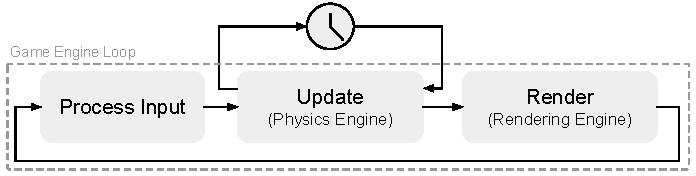
\includegraphics[width=0.5\textwidth]{Other/Figures/GameEngineLoop.pdf}
\caption{Game engine loop block diagram~\cite{GameProgPatternsBook}}
\label{GameEngineLoopDiagram}
\end{figure}
The first part of the game loop is to process the user inputs which may take the form of user keyed inputs or, in the case of CAV development, the resultant actions of the autonomous vehicle given the current state of the environment. For example, the throttle and steering inputs from the vehicle controller of an AV.
%
The update interprets the intended actions of all dynamic actors in the scene, performs any necessary physics calculations and updates the actor states. 
%
The rendering engine then takes the updated actor states and renders the scene~\cite{GameProgPatternsBook}. 
% 
% It is necessary to have an understanding of how the game loop operates in order to understand potential sources of non-determinism that are discussed below. 
% 
The key aspects of the game loop needed for this discussion are as follows: 

\begin{itemize}[leftmargin=*]
    \item At the beginning of each tick, the lag between the game clock and the real world is updated based on how much real time passed. This measures how far the game's clock is behind compared to the real world.
    \item Then the user inputs are processed.
    \item There is then an inner loop to update the physics processes (clock symbol in Fig.~\ref{GameEngineLoopDiagram}), incrementing at a delta time step, $dt$, until the game clock is equal to the real world. 
    \item Rendering occurs once the game clock has caught up with the real world clock. 
    \item The process then repeats.
\end{itemize} 

If the physics engine uses a fixed time step ($dt$), %, because it makes everything simpler and more stable for physics and AI.
the shorter this time step is the smoother the interpretation of the physical dynamics will be. %processing time it takes to catch up to game clock. % and the more deterministic the engine becomes and vice versa, as will be explained in section \ref{s:nondeterminisimSources}. 
%
To use a fixed physics time step the user's display refresh rate needs to be known in advance. This requires an update loop to take less than one render tick (one frame of real world time). Given the range of different hardware capabilities a variable delta time is often implemented for game playing taking the previous frame time as the next $dt$. However, variable $dt$ can lead to different outcomes in repeated tests and in some cases unrealistic physical representations~\cite{gaffer}. Semi-fixed or limited frame rates ensure $dt$ does not exceed some user-defined limit to meet a minimum standard of physical representation but allows computational headroom for slower hardware. Some engines provide sub-stepping which does multiple physics calculations per frame at a greater CPU cost~\footnote{\url{https://docs.unrealengine.com/en-US/Engine/Physics/Substepping/index.html}}. If the engine tries to render between updates \textit{residual lag} can occur and extrapolation between frames is performed to smooth transition between scenes, see lower part of Fig.~\ref{GameEngineLoopDiagram}. %\cite{GameEngineArchBook}\cite{GameProgPatternsBook}
%
% Ideally the time step should be as short as possible, so that the simulation returns better accuracy of complex physical processes. %runs with high fidelity on fast machines. 
In exceptional cases where resources are scarce, the fixed time step can be greater than the time between render ticks %it takes to process an ``Update" inner loop on some (slow) machines, 
and the simulation will exhibit lag between input commands and rendered states resulting in unsynchronised and unrealistic behaviour.

% The time step, $dt$, in the physics calculation is important and the smaller the value the more realistic the simulation will be. If $dt$ is too large or irregularly spaced then the rendered motion may not be smooth and interpolation may be required at additional computational cost. 

% This process allows hardware scalability, but the rendering will become of jerky quality on slower machines. These engines update at fixed intervals and render whenever they can, which is not steady. This results in what is so called residual lag\cite{GameEngineArchBook}\cite{GameProgPatternsBook}, where the engine is trying to render between two consecutive updates. In this case, the engine will use extrapolation techniques to give an estimate of where the object should be. This often is sufficient for gaming purposes and unnoticeable to the user, in fact it improves the stuttery motion.

\begin{figure*}[b]
    \centering
    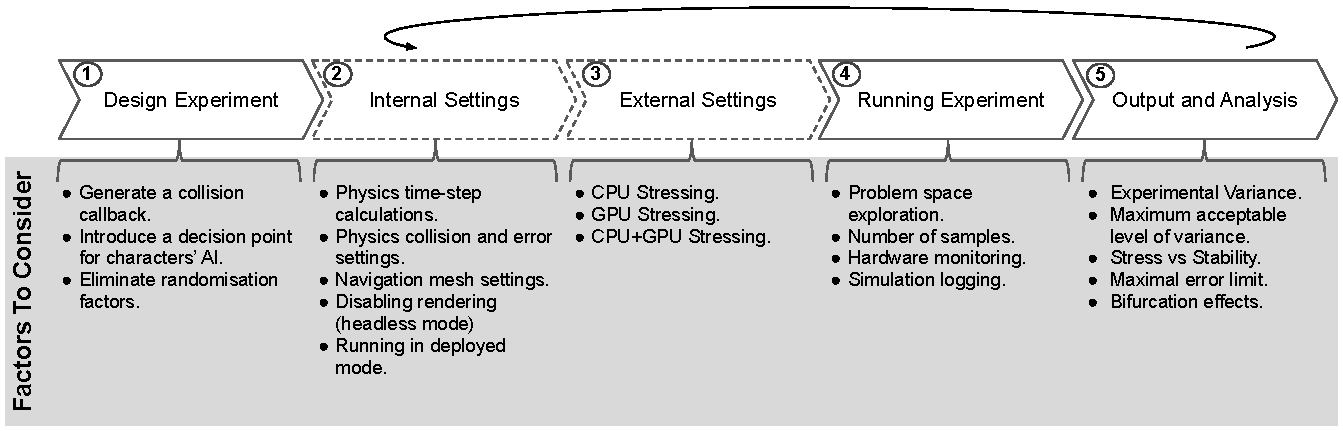
\includegraphics[width=0.99\linewidth]{Other/Figures/MethodologyDiagram.pdf}
    \caption{Shows a flow diagram of the methodology proposed to define the simulation variance of a gaming engine for usage in CAV simulations.}

    \label{method_diagram}
\end{figure*}

% ======= Sources of non-determinism
\subsection{Sources of Non-Determinism} \label{s:nondeterminisimSources}

The following points form a hypothesis around the potential sources of non-determinism that could occur in game engines. \\\\
% \noindent After establishing an understanding of how physics engines work, the focus will now be on what causes these engines to be non-deterministic. The main reasons that we think are causes of these engines' non-determinism are discussed below. \\\\

\noindent\underline{\textit{Floating Point Representation:}}
Floating point representation of real numbers is limited with fixed register sizes resulting in errors of \textit{rounding} where loss of bits occur which are rounded or truncated and \textit{cancellation} which happens where two similar values are subtracted~\cite{FloatingPointsBook,goldberg1991every}. 
%
% Translating to the usage of CAV simulations in physics engines,
This could result in precision issues of, for example, actor position within the environment and falsely satisfying or failing assertions. Such reasons would often make one jump to conclude that floating points are the cause of non-determinism, but these precision issues should be referred to as \textit{incorrectness} and not non-deterministic. Since hardware is assumed deterministic, then the same hardware should produce the same \textit{incorrect} output for the same initial conditions. So, even if the output is incorrect due to floating point precision it should always be the same, given the same logical registers which conform to the same IEEE floating point standard~\cite{8766229}. Therefore, it is unlikely that floating point representation will contribute to \textit{simulation variance} for repeated tests on the same hardware.
%
% A generic issue with computers are floating points precision. 
%Various errors occur when doing arithmetic manipulations using floating points, especially when operating between large and small numbers due to rounding, memory limitations and so forth.\cite{FloatingPointArithmeticArticle}\cite{FloatingPointsBook}. 
%Translating to the usage of CAV simulations for V\&V in physics engines, this could result in many precision issues resulting in complex non deterministic behaviours.
%
% For instance, consider a simulation where the world is infinite and progressively  generated in the physics engine. 
% After a few hundred meters, precision issues will start to occur, and will get progressively worse the further from the origin the simulation gets. 
% This is due to the values of the coordinates being used in calculations are getting bigger and hence will not cope with small values that are critical for V\&V testing purposes. 
% A solution to this problem is perhaps every time the simulations moves 100 meters away from the origin the entire world will move by 100m in the opposite direction. Thus, avoiding getting into floating point issues.\cite{FloatingPointArithmeticArticle}
%
% There are many scenarios that could be addressed, and solutions to them will entirely depend on the characteristics of that specific scenario. There is no generalised solution for the floating problem, regardless of how good computers get there will always be a limitation. However, floating points as they stand could just be sufficient for V\&V testing purposes. Whenever they are not, smart solutions can be found to accommodate for these limitations.
\\\\
\noindent\underline{\textit{Scheduling:}} %
Scheduling is a resource management method for sharing computational resources between tasks of different or competing priority where tasks are executed  dependent on the scheduler policy. A scheduler policy may be optimised in many ways such as for task throughput, deadline delivery or minimum latency~\cite{liu1973scheduling}. 
%
If during simulation the scheduling policy was updated or thread priority was inconsistently handled then variance in output may be expected. It is, however, unlikely that such events would occur on repeated controlled tests for the same hardware and operating system configuration. %
%
Similar to thread scheduling, the CPU scheduling policy determines which processor core to execute processes in the ready queue and this is maybe ordered by factors such as throughput, latency and CPU utilisation. %
%
If the same single-threaded script executes multiple times across different physical cores due to the CPU utilisation policy then should this be considered deterministic? Processor designs should be identical although impurity inconsistency across the bulk silicon and minor perturbations in the semiconductor processing across the chip may exist. End users expect such minor variations to be controlled for in architecture design and factory testing.

Another issue to consider is concurrency, where sequential tasks can be executed out of order to improve speed by utilising parallelisation although it depends on the decomposability of the program. This technique can lead to issues such as shared resource access conflicts and RACE conditions~\cite{huffman1954synthesis}. 


Scheduling of threads may be a reason for non-deterministic simulation behaviour in game engines. Given the same hardware the output should always be the same, unless scheduling of the threads change. 
% i.e. the utilisation of hardware is manipulated differently each time. This would then result in non-deterministic behaviours especially if it is combined with the floating point problem discussed earlier. 
%
% For example, if a process on thread 1 requires data from thread 2, but thread 2 is delayed due to additional load then synchrony between the threads may be lost if not controlled for explicitly. Given that game engines will promote performance over accuracy the process on thread 1 may be dropped or skipped until the data are available. This may lead to events happening out of order depending on the computational load and hence non-deterministic.
%
% To solve the scheduling of threads problem, one would have to control all of the threads during runtime, which is very involved. To achieve that one would need to replace or control the whole run-time system to allocate tasks to the same threads in the same order. This is beyond the scope of our work and will not be covered in this paper.
\\\\
\noindent\underline{\textit{Physics and Rendering clocks:}}
% The inherent way of how these physics engines operate (i.e.game loops) causes the engine to be non-deterministic.  A follow up from section \ref{GameLoopSection}, these
Some game engines use a variable frame rate, which is good for hardware scalability but creates a challenge for the physics engine which works best with small fixed time steps. %
%
The problem of having a variable frame rate could also contribute to the non-deterministic behaviour of these engines, especially combined with loss of thread scheduling synchrony. 
%
That is to say, if the frame rate is allowed to vary then it has to be controlled to give the same variability through out a given test in order for the test results to be repeatable. This issue might be of negligible significance if the frame rate is consistent and the time steps are small enough. 
\\\\
\noindent\underline{\textit{Actor Navigation:}}
Game engines often use navigation meshes for actor path planning, which should be considered as a potential source of non-deterministic behaviour, e.g.%. Some CAV simulator developers claim that the built-in physics engines' AI is non-deterministic
~\cite{CARLABenchmark}. 
This may depend on the algorithms used by the engine which typically use the A* algorithm\cite{AStarBook} and should give deterministic outcomes as long as the environment is deterministic\cite{AirsimUnrealArticle}\cite{UnrealAIDocumentation}. 
Therefore, the determinism of the actor path planning depends on the environment and the update to actor states within it and how navigation meshes are created or modelled, e.g. shape, granularity. 
%
It is interesting to note that changes can occur to navigation meshes if they are dynamically loaded as the simulation proceeds which can reduce computational load for large area maps~\footnote{\url{https://docs.unrealengine.com/en-US/BlueprintAPI/AI/Navigation/RegisterNavigationInvoker/index.html}}. %This non-deterministic behaviour can be also resorted to the different scheduling of threads, hence giving variations in meshes every time they are loaded.



% %
% \section{Methodology} \label{method}
\noindent A method for determining the level of non-determinism of an engine is presented in this section and the working flow of the method is shown in Figure \ref{method_diagram}. Each of the steps in the method is elaborated in the following subsections.
\begin{figure*}[h!]
    \centering
    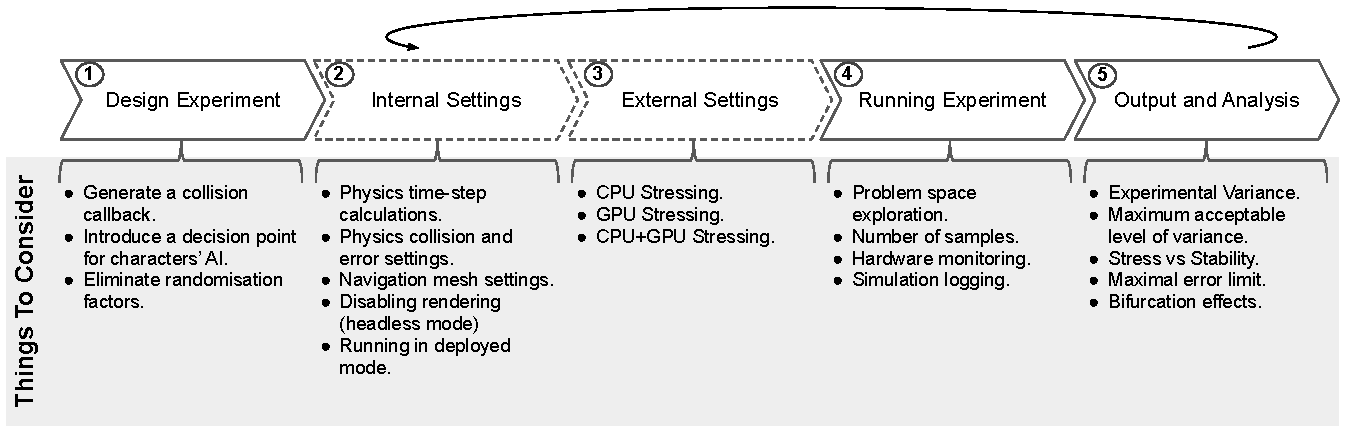
\includegraphics[width=0.99\linewidth]{Other/Figures/MethodologyDiagramCropped.pdf}
    \caption{Shows a flow diagram of the methodology proposed to define the level of non-determinism of a physics engine.}

    \label{method_diagram}
\end{figure*}
\subsection{Design experiment}
\noindent When designing the experiment(s) one needs to bare in mind the following two questions: i) Is the engine deterministic? ii) If not, how does its level of non-determinism vary?\\\\
In simulation, actors can either follow a series of trajectory way points or they get given the destination and their AI path plans to that destination. 
Thus, given that an engine is non-deterministic one needs to set up an experiment that would stress the engine in order to determine how its level of non-determinism vary. This is best done by generating collision callbacks, because that is when engines' do a lot of calculations to determine the response after the collision. Another approach, if AI is used for path planning instead of just following predefined trajectory way points, is to introduce a decision point for the AI.\\\\
It is crucial to also make sure that any randomisation factors are eliminated in the experiment.

\subsection{Internal settings}
\noindent There are several error and physics collision internal settings in physics engines that can be tweaked to enhance the level of non-determinism. \\\\
\noindent Increasing the physics time-step calculations, which is increasing the number of calculations per unit time, would improve the level of non-determinism since the physics sequence will be more finely defined; but on the other hand this would be more computationally expensive. However, in such applications of V\&V of CAV simulations, the computational cost should be of less concern compared to the importance of repeatability of tests. \\\\
\noindent If the experiment setup includes the usage of the physics engine's AI then altering the navigation mesh settings in the engine, like increasing the granularity of the mesh or changing the mesh type; can improve the level of non-determinism as a result of allowing the AI to navigate in a more well defined space.  \\\\
\noindent Disabling rendering or running in headless mode is a way of attempting to decouple the rendering engine from the physics engine, which theoretically should affect positively the repeatablility of tests. 
The downside of most physics engines is that they do not provide a headless mode in the editor setup, thus this could make running in headless mode a real challenge for verification engineers.  \\\\
\noindent Running in editor or deployed mode can sometimes cause massive differences in performance, with deployed mode being worse, mostly due to the way settings get packaged when in deployed mode.

\subsection{External settings}
\noindent Running other programs in the background, like having a web browser open, or running the physics engine in the background while performing other tasks on the same machine does also have an effect; because it alters the CPU and GPU utilisation of tasks.\\\\ 
\noindent Trying to run stress experiments on computers by running other programs makes it difficult to control experiments since the utilisation would be inconsistent, nonetheless, there exists dedicated stress utilisation programs which provide consistent CPU and GPU stressing. Note, however, that during running these tests computers should be left alone not be used for any other purposes apart from running the experiments.

\subsection{Running experiment}
\noindent When it comes to running the experiment itself, things that one should consider  are the problem space exploration; the number of runs that should be executed to get reliable results; the frequency of logging data of actors; and possibly having a program to monitor the hardware utilisation.
% Problem exploration, there is too many variables that one can play with. do statistical analysis some.... some of them get problematic...

\subsection{Output and analysis}
\noindent Once the experiments are run, the logged data is post processed to find the variance in the logged data between the different runs. Note that bifurcation effects can cause a jump in the variance, so it is worth plotting the different logged paths in order to determine if there are any bifurcation effects.\\\\
This whole process is repeated for various internal and external settings. 
Then various plots can be created to identify and engine's level of non-determinsim. 
Thereon, it would be up to the verification engineers to determine where they want to define the line below which the level of non-determinism would be acceptable, and thus know at which levels of computational utilisation they can guarantee to run repeatable experiments.   


% %
% \section{Case Study} \label{s:case-study}
Given that our interest is on CAV simulations, this study presents a number of experiments run on typical agents used in CAV simulations and their interactions with each other. These agents are classified into two, either vehicles(cars, motorcycles, bikes etc.) or pedestrians (can include animals).

Here we will walk through our hypothesis, description of our tests and the analysis of results from the different tests. We will point out at each stage where we sit in Figure~\ref{method_diagram} as we go through this case study.    

\subsection{Problem And Hypothesis}
We want to see whether using Unreal Engine 4 (UE4) along with CARLA \cite{CARLA_paper} for V\&V of CAV simulations is deterministic or not; if not then what is the level of simulation variance that we will operate with, is it acceptable or not, and whether it worsens with stressing GPU and CPU.

Our hypothesis is that since UE4 is a gaming engine it is not deterministic, however, the level of simulation variance would be very low to acceptable limits that allows verification engineers to use it confidently and assume that tests would be repeatable.
This behaviour is expected not to hold as the level of computing stress increases.     

\subsection{Tests Description And Technicalities}\label{TestsDescriptionAndTechnicalities}
The vehicles in this simulator follow a trajectory of waypoints using a PID controller and they have a look ahead distance that they target for from a given list of trajectory waypoints. 
Similarly with the pedestrians, but they don't have a PID controller and they can do dynamic path planning using A* algorithm to reach their destination or in this case a trajectory waypoint.

Starting from step 1 in the methodology diagram (Design Experiment); we are using a double mini roundabout for our experiments. 
The list of tests shown in Table \ref{TableOfExperiments} were chosen to cover the mandatory interactions between the different types of agents. 
These are summed up in the following: \textbf{i)}Agents (vehicles and pedestrians) moving with no collisions or interactions with each other \textbf{ii)}Collision between vehicles \textbf{iii)}Collision (intersection) between pedestrians \textbf{iv)}Collision between vehicles and pedestrians.

\begin{figure}[h]
    \centering
    \begin{subfigure}{.24\textwidth}
        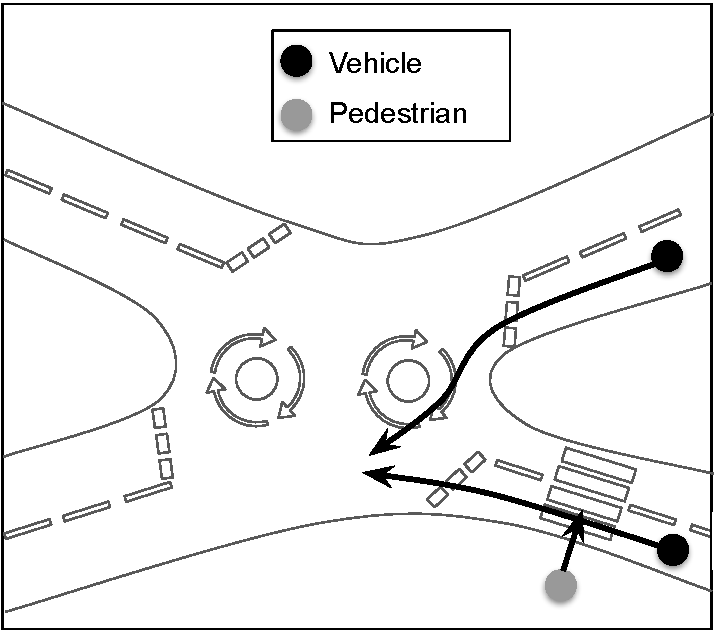
\includegraphics[width=1\textwidth]{Other/Figures/TestCasesDiagram_a.pdf}
        \caption{}
        \label{Test_a}
    \end{subfigure}
    \begin{subfigure}{.24\textwidth}
        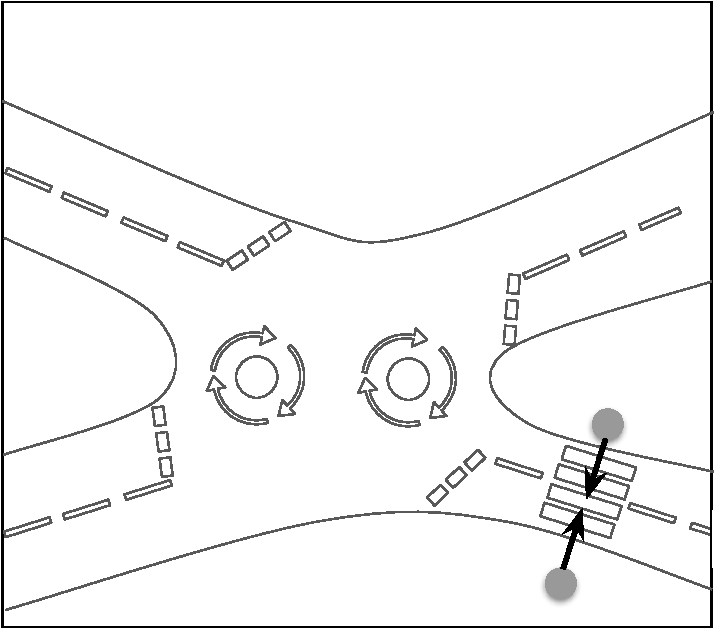
\includegraphics[width=1\textwidth]{Other/Figures/TestCasesDiagram_b.pdf}
        \caption{}
        \label{Test_b}
    \end{subfigure}
    \caption{Shows the setup of the different tests in Table \ref{TableOfExperiments} (a)Test IDs 1 to 4 (b)Test IDs 5 to 8.}
\end{figure}

Tests 1, 3and 5 are similar and there are no collisions in them, they were done as separate tests (instead of combining them into one) for the sake of simplicity and to use them as base lines for the tests-collision versions of them. The tests for collisions and non-collisions differ by a very slight change in the trajectory of the agents just to make them avoid colliding or intersecting with each other.

Test 2 is a collision between two vehicles and no pedestrians involved and is depicted by \ref{Test_a}, where the two vehicles will approach the roundabout and crash.

Tests 6,7 and 8 are tests with pedetrians having the same trajectory waypoints but walking in opposite directions to each other (see Figure~\ref{Test_b}). 
Pedestrians have the functionality of dynamic path planning i.e. they can avoid obstacles to reach their waypoints and so they can avoid bumping into each other. 
Hence, to make sure they intersect (collide) with each other then we  have set tests 6,7 and 8 to be the same but with different look ahead distances; the smaller the look ahead distance the less chance they will get to path plan around each other, and thus making sure they intersect.

In V\&V of CAV simulations, collisions of pedestrians together is not of much interest, nevertheless we decided to include these tests for the sake of completeness and to obtain a full image of the simulation variance of the simulator.

Test 4, is where a vehicle hits a pedestrian and runs over it on a zebra line, as shown in Figure~\ref{Test_a}.

Proceeding to step 2; there is about 20 different internal settings related to our context that can be tweaked in UE4; such as \textit{Enable Enhanced Determinsim}, \textit{PhysX Tree Rebuild}, \textit{Max Physics Delta Time} etc. By doing various inspections around them we did not notice much improvement or worsening in the simulation variance between test runs, therefore the internal settings option was disregarded.

On the other hand the external settings (step 3), where CPU + GPU are stressed, did show significant variations in the results as will be discussed in section \ref{ResultsSection}.
Different levels of stress were applied to the computer; using the \texttt{stress} function \cite{CPU_stress} to stress the CPU and \texttt{gpu-burn} from github \cite{GPU_stress} to stress the GPU.

In terms of running the experiments (step 4), \textbf{i)} the computer used is an Alienware Area 51 R5 with an i9 9960X CPU chip, NVIDIA GeForce RTX 2080 graphics card and 64GB of RAM; \textbf{ii)} \texttt{nvidia-smi} and \texttt{htop} were used to monitor the levels of GPU and CPU stress respectively before and while the experiments were executed \cite{monitoring_stresses}; \textbf{iii)} the computer was left alone and not used for any other tasks while the runs were executed.

\subsection{Results And Discussion}\label{ResultsSection}
We start by analysing (step 5) the summary from all of the tests plotted in Figure~\ref{ExperimentsStressSummary}; where the x-axis represents the percentage of CPU + GPU utilisation and the y-axis shows the total mean devaition. 
This was calculated by averaging the variance between all of the different runs through out the simulation time for all of the agents, then taking the square root to obtain the total mean devaiton.
\begin{figure}[h]
    \centering
    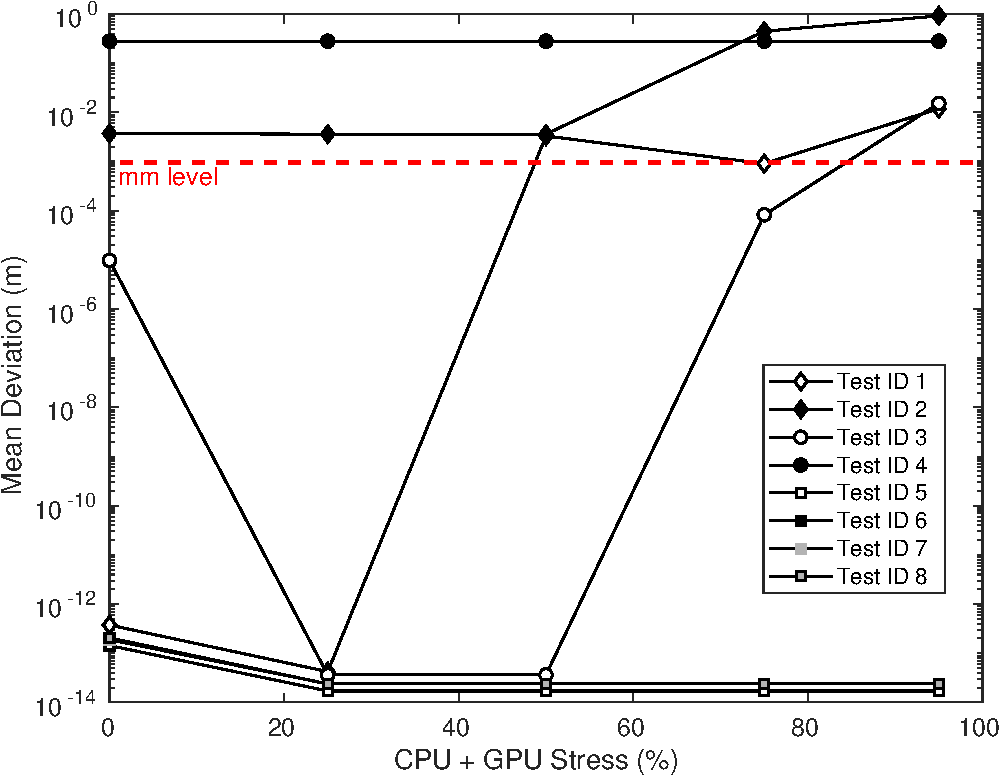
\includegraphics[width=0.48\textwidth]{Other/Figures/ExperimentsStressSummary.pdf}
    \caption{Summary of total mean deviation for the different tests runs plotted against the different CPU + GPU stresses.}

    \label{ExperimentsStressSummary}
\end{figure}

\begin{figure*}[h]
    \centering
    \begin{subfigure}{.49\textwidth}
        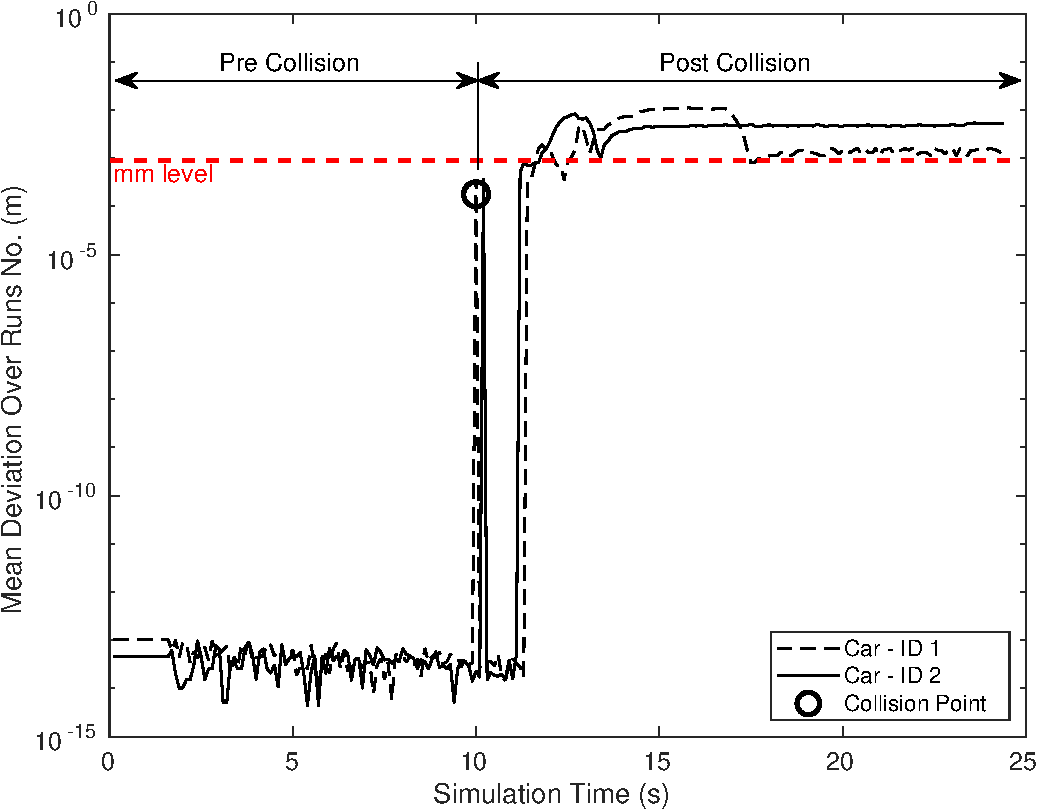
\includegraphics[width=1\textwidth]{Other/Figures/CarsCollisionCG25.pdf}
        \caption{}
        \label{CarsCollisionCG25}
    \end{subfigure}
    \begin{subfigure}{.49\textwidth}
        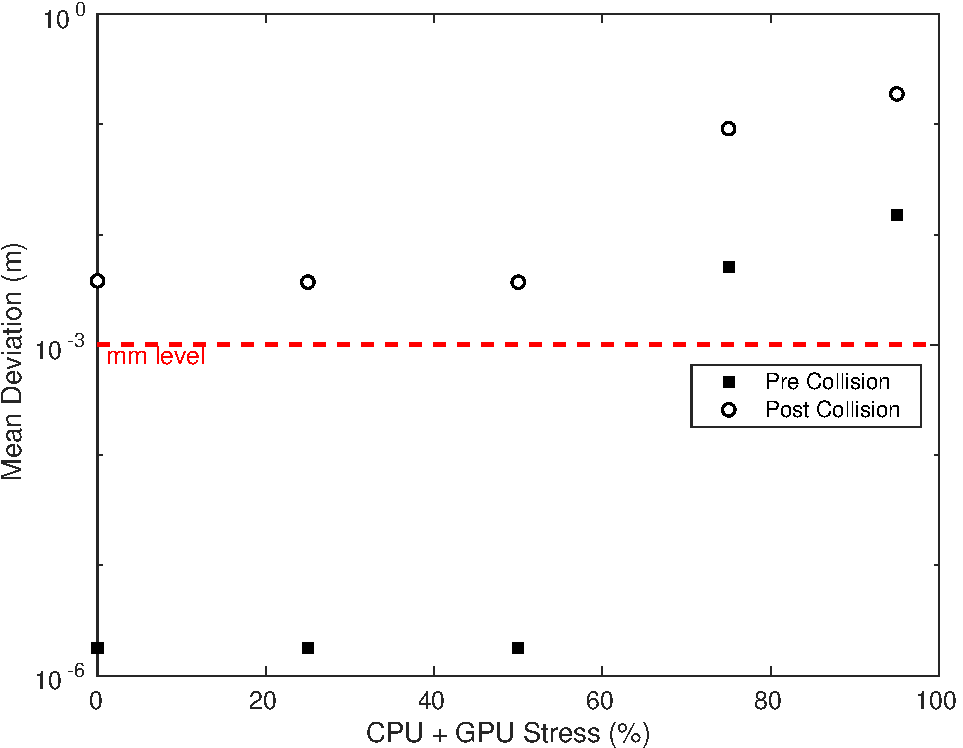
\includegraphics[width=1\textwidth]{Other/Figures/CarsCollisionPrePost.pdf}
        \caption{}
        \label{CarsCollisionPrePost}
    \end{subfigure}
    \caption{Test ID 2 (a)Mean deviation over runs no. vs simulation time for 25\% stress. (b)Pre and post collision mean deviation over runs no. for different CPU + GPU stresses.}
\end{figure*}

\begin{figure*}[h]
    \centering
    \begin{subfigure}{.49\textwidth}
        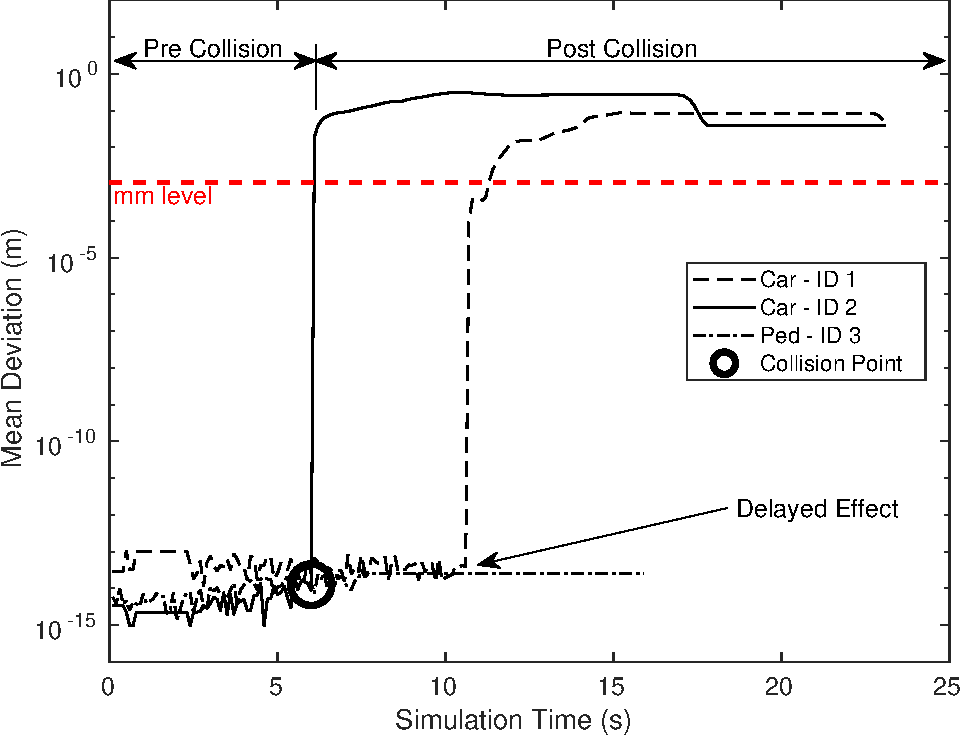
\includegraphics[width=1\textwidth]{Other/Figures/CarsPeopleCollsionsCG25.pdf}
        \caption{}
        \label{CarsPeopleCollsionsCG25}
    \end{subfigure}
    \begin{subfigure}{.49\textwidth}
        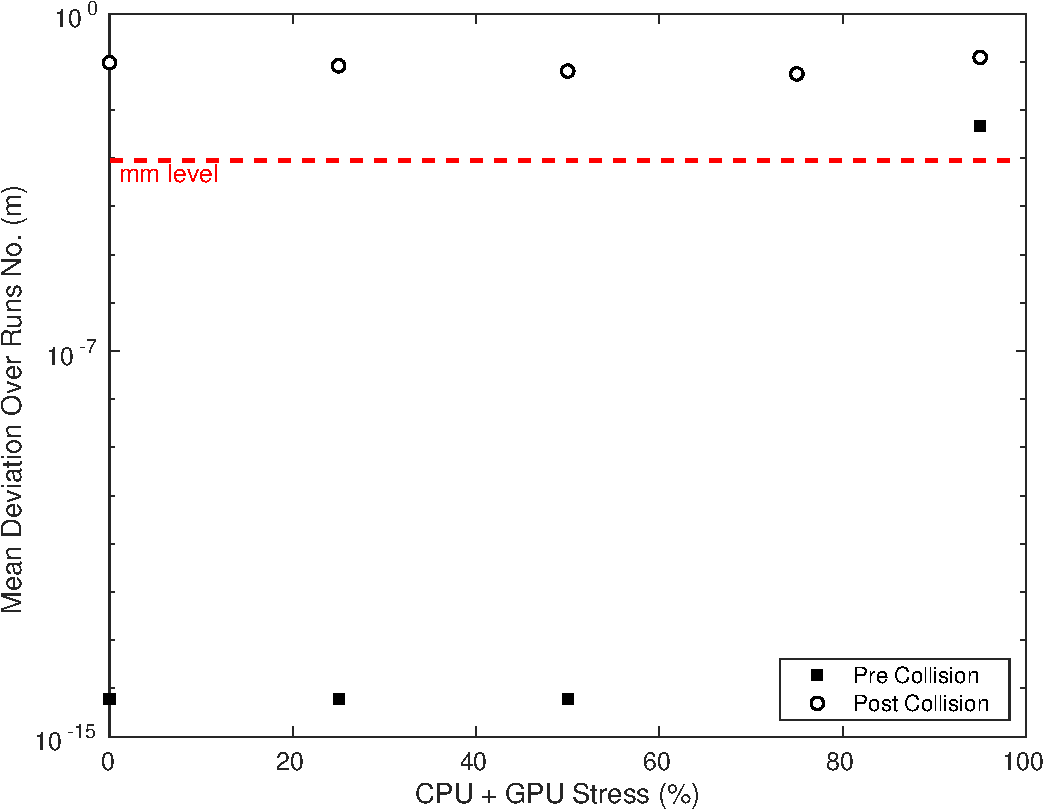
\includegraphics[width=1\textwidth]{Other/Figures/CarsPeopleCollisionPrePost.pdf}
        \caption{}
        \label{CarsPeopleCollisionPrePost}
    \end{subfigure}
    \caption{Test ID 4 (a)Mean deviation over runs no. vs simulation time for 25\% stress. (b)Pre and post collision mean deviation over runs no. for different CPU + GPU stresses.}
\end{figure*}
Note the dotted red line in the plot shows the millimeter (mm) level. 
Below this level we assume that the level of simulation variance is very low for V\&V of CAV simulations purposes, that it is sufficient to assume the tests are deterministic and repeatable. 
This line can be moved up or down and it is entirely up to verification engineers where they want to define the level below which tests' variance is negligibale and it is suffcient to assume that tests are deterministic, but just for the sake of argument we chose it to be the millimeter level.


First, the tests with no collisions are considered, these represent tests 1, 3 and 5.
Tests 1 and 3, which involves vehicles only and vehicles with pedestrians respectively, shows very low simulation variance for stress levels below 50\% and as the stress level increases they surpass the red line crossing our defined deterministic level but still being sufficiently low (i.e. with in the centimeter level). This clearly shows how the load on a computer (i.e. stressing CPU and GPU) can have drastic effects on the repeatablitiy of tests.
This is more specific to vehicle agents rather than pedestrians since the behaviour of pedestrians is consistent and remarkably below the mm level for all of the different levels of stress shown by test 5, where only pedestrians are involved with no collisions, from which it can be deduced that the mean deviation change with the stress level in test 3 was solely due to the vehicles.

Next, given the pedestrians were showing a very robust and low level of simulation variance, we ran tests for pedestrians colliding (i.e. with paths intersection) for different look ahead distances to exploit whether that would cause any changes, but yet as it can be seen by lines Test IDs' 6,7 and 8 that their performance is consistent for all of the different tests.

Finally, we look at the other collisions tests, tests 2 and 4 where the tests correspond to a collision between two vehicles and a collision between a vehicle and a pedestrian respectively. 
We observe that in both of these tests the mean deviation is always above our red line regardless of the stress level, nevertheless still increasing the stress levels shows worsening effects.

Thus, we resorted to plotting the mean deviation over the number of runs of these two tests vs simulation time with stress level \%25 chosen arbitrarily (see Figure~\ref{CarsCollisionCG25} and \ref{CarsPeopleCollsionsCG25}). 
Doing that we discovered that after collisions occur there is a jump in the mean deviation, which is what causes the averaged mean deviation through the whole simulation time in Figure~\ref{ExperimentsStressSummary} to always surpass our red line.

Plotting Figures~\ref{CarsCollisionPrePost} and \ref{CarsPeopleCollisionPrePost}, which shows the mean deviation pre and post collision for the different stress levels; it can be seen that there is two discrete levels for the pre and post collison devaition from these plots and as the stress increases these two discrete levels start to merge. 
However, in V\&V of CAV simualtions we  are normally interested in the point until a collision occur after which the simulation will be terminated. Thus, the post collision effect should not be of much concern in the context of CAVs.
It is important to note, however, that in test 4 a delayed effect of increase in simulation variance was noticed to Car ID 1, which interestingly was not involved in the collision, this was attributed to how the physics engine was programmed to calculate collisions which might cause other obscure behaviours to other agents. The importance of this outcome is that it shows even if an ego vehicle is not involved in a collision, but other agents are, this will still have effects on the simulation variance of the ego vehicle. Thus failing to stay below our red line and the test should be terminated.
In summary, from the tests carried out we can deduce that for a computer of the following specifications, an Alienware Area 51 R5 with an i9 9960X CPU chip, NVIDIA GeForce RTX 2080 graphics card and 64GB of RAM, that all tests carried out using CARLA in UE4 are gauranteed to be deterministic and repeatable (according to our definition by the red line) as long as the CPU + GPU stress does not exceed 50\% and tests are terminated as soon as a collision of any type is detected in the simulation. 
% %
% % \input{5_ResultsAndDiscussion.tex}
% %
% \section{Conclusions}\label{s:conclusion}
We have provided a summary of the sources of non-determinisim in game engines. This was followed by presenting a method by which one can determine the simulation variance of a gaming engine used in V\&V application of CAV simulations. The method consists of five stages, starting with designing the experiment, then suggesting the various settings that can improve or worsen the performance, and finally focuses on running the experiment and analysing the output.

A case study is then used to show the implementation of the method introduced, where several tests were setup and run to explore the different interactions between the different agents in a simulator called CARLA. It was found that for the computer used (with specs of an i9 9960X CPU chip, NVIDIA GeForce RTX 2080 graphics card and 64GB of RAM) the simulation variance was sufficiently low to assume the simulator to be deterministic as long as the CPU + GPU utilisation is below 50\% and that tests are terminated as soon as a collision of any type is detected. %since it was noticed that collisions cause the level of non determinism to jump remarkable invalidating the assumption of the simulator is deterministic.

In highlight of obtaining a fully determinstic simulator, one would either have to explore methods to control the scheduling of threads in a computer such that if tests are rerun the utilisation of hardware will be the same. Alternatively, another approach would be to create a new engine that is designed to be deterministic with minimal attention given to performance. 



% %
% 

\section*{Acknowledgements}
\noindent This work is part of the ROBOPILOT and Capri projects funded by Innovate UK.
% \textbf{Competition Name:} Connected and Autonomous Vehicles 2.\\ 
\textbf{Competition Code:} 1608\_CRD1\_TRANS\_CAV2S1


\printbibliography
% %

% ***************************************************
%  TITLE
% ***************************************************
\title{Investigating Determinism of Game Engines for Autonomous Vehicle Verification}
\author[1,3]{Abanoub Ghobrial\thanks{$^{1}${\footnotesize \{abanoub.ghobrial, greg.chance, kerstin.eder\}@bristol.ac.uk}}}
\author[1,3]{Greg Chance}
\author[2,3]{Severin Lemaignan\thanks{$^{2}${\footnotesize \{severin.lemaignan, tony.pipe\}@brl.ac.uk}}}
\author[2,3]{Tony Pipe}
\author[1,3]{Kerstin Eder}
\affil[1]{Trustworthy Systems Lab, University of Bristol, Bristol, UK}
\affil[2]{University of West of England, Bristol, UK}
\affil[3]{Bristol Robotics Lab, Bristol, UK}
\maketitle

\begin{abstract}
\noindent 
The autonomous vehicle (AV) community is adopting the use of game engines to develop vehicle control systems and testing environments using simulation. Determinism is a key requirement for simulation during AV development and testing. In particular, it ensures repeatability of tests, so that software bugs can be found and fixed, and simulation results are trustworthy.
%
% KIE: Ideally, these engines are deterministic, but we've found that they are not. :(
% These engines must be deterministic for finding and resolving defects (bugs) in software and ensuring auditable and repeatable tests can be executed for verification and validation (V\&V). 
%
However, game engines do not need to be deterministic per se. % when used for games. 
%
This work identifies the requirements these engines need to fulfil when used for AV development and testing, and proposes a method to determine the \textit{simulation variance} for specific configurations and utilisation of the software and hardware, respectively. 
%
A case study using Carla, an open-source simulation environment powered by Unreal Engine, illustrates the proposed method and results from a small scenario indicate the presence of deterministic operational domains. \todo[inline]{KIE: review at end}

% The industry and certification bodies for connected autonomous vehicles is adopting the use of physics and gaming engines to develop, train, verify, validate and certify the software of these autonomous systems in simulation. It is important for these engines to be deterministic in order for one to carry out these different processes. However, such engines are inherently non-deterministic. We propose a method by which one can identify the region where they can operate in these engines and guarantee that the level of non determinism is sufficiently low that it can be assumed to be deterministic. We also implement this method on a case study and show how we identified the region (encompassing computational utilisation and behaviours in simulation) at which one can guarantee performance to be sufficiently deterministic.          
\end{abstract}

\begin{IEEEkeywords}
Autonomous Driving, Determinism, Physics Engines, Autonomous Vehicles, Verification and Validation (V\&V), Simulation, Testing
\end{IEEEkeywords}
\IEEEpeerreviewmaketitle

% ***************************************************
%  INTRODUCTION
% ***************************************************
\section{Introduction} \label{s:introduction}
% What is verification
\IEEEPARstart{V}{}erification is the process used to gain confidence in the correctness of a system with respect to its requirements~\cite{bergeron2012writing}. Simulation based verification can be used to test autonomous driving functions under development benefiting from full control over the road network and the actors within it. These simulated tests aim to provide evidence to developers and regulators of the functional safety of the vehicle or its compliance with commonly agreed upon road conduct~\cite{ViennaConv}, national rules~\cite{codes2015highway} and road traffic laws~\cite{RoadTraffic1988} which form a body of driving assertions that must not be violated. 

Design confidence is gained when the autonomous vehicle (AV) can be shown to comply with these rules, e.g.\ through assertion checking during simulation. 
There have been a number of fatalities with AVs, some of which could be attributed to insufficient verification and validation (V\&V), e.g.~\cite{FatalityExample}. Simulation environments offer a means to explore the vast parameter space in a safe and efficient manner~\cite{korosec2019waymo} without millions of miles of costly on-road testing~\cite{kalra2016driving}. In particular, simulations can be biased to increase the frequency at which otherwise rare events occur~\cite{Koopman2018}; this includes testing how the AV reacts to unexpected behaviour of the environment~\cite{RobustnessAutonomy}. 

% The use of game engines for AV testing
Increasingly, the autonomous vehicle (AV) community is adopting game engines as simulation platforms to support the development and testing of vehicle control software. 
%
Carla\footnote{http://carla.org/}, for instance, is an open-source simulator for autonomous driving that is implemented as a layer over the Unreal Engine (UE4), a  real-time 3D creation environment for the gaming and film industry as well as other creative sectors~\cite{CARLA_paper}. 

% Requirements of simulation based verification SBV
The benefit of using state-of-the-art game engines as simulators is that they offer sufficient realism~\cite{Koopman2018} in the physical domain combined with realistic rendering of scenes, potentially suitable for perception stack testing and visual inspection of accidents or near misses. 
%
Furthermore, they are easy to setup and run; they also are simple to control and observe, both with respect to the environment the AV operates in as well as the temporal development of actors~\cite{Ulbrich2015}. 
%
For game engines to be used in simulation-based testing of AVs, they must offer sensors that operate at an accuracy equivalent to those on the AV, e.g.\ video cameras, LIDAR, IR, etc., or interfaces for developers to integrate their own sensor models. Carla currently offers various basic types of cameras and ray-case based lidar; extensions are still under development. 
%
Finally, support for hardware-in-the-loop development or a real-time test-bed for cyber-security testing~\cite{Javaid2013} may also be required. 

% Game engines for SBV
Compared to the vehicle dynamics simulators and traffic-level simulators used by manufacturers~\cite{FrameworkAndChallenges}, game engines offer a convenient simulation solution that meets many of the requirements for the development and functional safety testing of AVs in simulation. However, several challenges remain; one of these is determinism.
%
% What is a deterministic system
Deterministic, in this context, refers to the property of causality given a temporal development of events such that any state is completely determined by prior states.
%
Herein the term \textit{simulation variance} is used to refer to how simulation traces and outputs vary, when the same stimulus is provided repeatedly under identical conditions. Specifically, we focus on the variance of actor paths within a given scenario. 

We will adopt the terminology defined in~\cite{Ulbrich2015}, where \textit{scene} refers to all static objects including the road network, street furniture, environment conditions and a snapshot of any dynamic elements. Dynamic elements are the elements in a scene whose actions or behaviour may change over time; these are considered actors and may include other road vehicles, cyclists, pedestrians and traffic signals. The \textit{scenario} is then defined as a temporal development between several scenes which may be specified by specific goals and values.\todo[inline]{values - Does this mean stimulus or other parameters?} A \textit{situation} is defined as the subjective conditions and determinants for behaviour at a particular point in time.

% Verification and Determinism 
% Why is determinism important for verification
%For game engines to be useful as a verification tool then they must be deterministic. -> any sim tool must be deterministic, not just game engines ;)
Determinism is a key prerequisite for simulation during AV development and testing. 
%
A deterministic simulation environment guarantees that tests are repeatable. 
%
Thus, coverage results are stable and, when a test fails, debugging can rely on the test producing the same trace and outcome when repeated. This ensures that software bugs can be found and fixed efficiently, and that simulation results are trustworthy. 
%
%Any software defects that are detected but not repeatable at a later time or by another party does not allow for suitable resolution. Furthermore, defects not found on the verification testing system may arise on a deployed system with a different hardware architecture resulting in untested and potentially unsafe behaviour. 
%When considering the development of autonomous vehicles, untested code could lead to dangerous behaviours not being identified and fatal road accidents may occur.
%
If the simulation is not deterministic, however, variance in actor positions, for instance, may lead to assessment errors, making it difficult to understand and remove bugs. In the worst case, bugs that could have been identified in simulation are left undetected, resulting in false confidence in the safety of the AV's control software.

% Challenges of SBV
Game engines do not need to be deterministic when used for gaming; there are no safety implications from non-determinism in this domain, nor is finding and fixing all the bugs a high priority for games developers. Because the situation is very different for AV development and testing, our main research question is: 
how can one assess the extent to which a simulation environment is deterministic? 
%
In pursuit of an answer to this question we have developed a method to determine the simulation variance for a given simulation environment. 
%
Knowing the simulation variance will help developers and testers understand the impact of using a game engine for AV simulation, especially how potentially existing non-determinism affects repeatability and reliability.\todo[inline]{review and potentially summarize results from case study}
%
%The game engine, in this context, must also comply with the requirements to provide a suitably realistic environment and real-time processing for perception and security analysis.\todo[inline]{next}

This paper is structured as follows. In Section~\ref{s:background} game engines and sources of potential non-determinism in game engines are investigated. Section~\ref{s:methodology} presents a method to assess the suitability of a simulation system for AV verification. 
%
A case study to illustrate how the simulation variance observed for a number of scenarios is presented in Section~\ref{s:case-study}.\todo[inline]{point to UE4} We conclude in Section~\ref{s:conclusion} and give an outlook on future work.\todo[inline]{review at end}


% \noindent \IEEEPARstart{T}{}he evolution and inevitable implementation of connected and autonomous vehicles (AVs) on roads is a delicate if not utterly fascinating subject. Such systems operate in environments marked by inaccessibility, unexpected weather conditions, or unpredictable behavior by surrounding humans\cite{RobustnessAutonomy}. 

% Public safety is clearly a prime concern for putting autonomous vehicles into play, which means the meticulous and thorough process of developing, training, verifying, validating and certifying the artificial intelligence (AI) and software of the vehicle is a task to be handled with care. 

% It requires lots of flexibility and room to iterate to ensure the algorithms are given the sharpest understanding for maximum performance as well as to ensure that they are hazard-free in order for them to be deployed\cite{AirsimUnrealArticle}.\\\\

% \noindent There has been a number of catastrophic fatalities with self-driving vehicles due to lack of verification and validation (V\&V) of software e.g.\cite{FatalityExample}.

% As such, there appears the need for finding ways to V\&V the safety of such software, ranging from AI development to cyber-security, while maintaining minimal risks in testing.\\\\

% ======================
% This is all from "FrameworkAndChallenges" without using quotes 
% \noindent Existing vehicle manufacturers use vehicle dynamic simulators to model the physics of each component in a system. Similarly, the use of simulation for traffic modelling is well established. Despite these proven simulation tools, non of them provide all of the required functionalities together to fully simulate AVs\cite{FrameworkAndChallenges}.\\\\

% While traffic-level simulators can model road layouts, they do not require as much realism or detail as AVs require. On the other side, vehicle dynamics simulators include some of the high fidelity physics functionalities needed for AV testing, but they only consider the vehicle itself and perhaps the road surface and gradient; they do not model any of the road layout, signs, traffic/street lights, other street furniture or surrounding infrastructure. 
% Most critically, neither types of simulators model sensors such as cameras, lidars or radars\cite{FrameworkAndChallenges}.\\\\ 
% Consequently, one of the major routes AVs developers are moving towards is using physics engines, these are often games engine development frameworks, since they tick all of the boxes needed to fully simulate AVs \cite{FrameworkAndChallenges}.  
% ======================

% Robopilot, Capri, Carla, Apollo, Airsim, Udacity etc. are all examples of driving simulator projects that use physics engines to support development, training, and validation of autonomous driving systems software\cite{ListOfSimulators}. \\\\
% Test-retest reliability, is a key factor in V\&V of software. Tests need to be repeatable in order for one to eliminate bugs. 
% In other words physics engines has to be deterministic, or the level of non-determinism of the engine should be low and clearly defined, for them to be used in the context of V\&V of AV software.\\\\
% \TODO{Remove this paragraph?} Determinism of game (physics) engines has not attracted much attention by engines' developers nor researchers. This previously was not important since in gaming, determinism is not critical. 
% Performance, on the other hand, is a subject of more interest in that field, where developers want games to work on all platforms and still be fast to provide a positive user experience. 
% On the contrary, determinism becomes vital and performance not when such engines are used in autonomous vehicles' AI development and testing. \\\\

% This paper aims to investigate how deterministic physics engines are for usage in V\&V for AV simulations; and will cover the list of following points:
% \begin{itemize}[leftmargin=*]
%     \item Necessary background on game engines used in AV simulations.
%     \item Review of sources of non-determinism in such engines.
%     \item Provide a method of how the level of non-determinism can be investigated and defined.
%     \item A case study showing the implementation of this methodology in an engine widely used in AVs simulations (Unreal Engine).
% \end{itemize}
 
% ***************************************************
%  BACKGROUND
% ***************************************************
\section{Background} \label{s:background}

There are numerous game engines with their associated development environments which could be suitable for AV development, e.g. Unreal\footnote{\url{https://www.unrealengine.com/}}, Unity\footnote{\url{https://unity.com/}}, CryEngine\footnote{\url{https://www.cryengine.com/}}. Specific autonomous driving research tools have been created to abstract and simplify the development environment, some of which are based on existing engines, e.g.\ Carla\footnote{\url{http://carla.org/}}, AirSim\footnote{\url{https://microsoft.github.io/AirSim/}}, Apollo\footnote{\url{http://apollo.auto/}}, and some have been developed for cloud based simulation, e.g.\ Nvidia Drive Constellation\footnote{\url{https://www.nvidia.com/en-gb/self-driving-cars/drive-constellation/}}.

Investigating the determinism of game engines has not attracted much research interest since performance is more critical for game developers than accurate and repeatable execution.  %However, when these engines are used for AV development then deterministic behaviour is required. 
This section gives an overview of the internal structure of a game engine and what sources or settings in the engine may affect \textit{simulation variance}.
%
% \noindent This section overviews important information and concepts in physics engines, which are relevant to their usage in AV simulations. Particularly, on how physics engines operate and the sources of non-determinism in these engines necessary to understand the contribution of this paper.

% ======= Overview of a Game Loop
\subsection{Overview of a Game Loop} \label{GameLoopSection}

Central to a game engine are the main game logic, the artificial intelligence (AI) component, the audio engine, and the physics and rendering engines. For AV simulation, we focus on the latter two.
%
The game loop is responsible for the interaction between the physics and rendering engines. Fig.~\ref{GameEngineLoopDiagram} depicts a simplified representation of the process flow in a game engine loop, where  initialisation, game logic and decommissioning have been removed\footnote{\url{https://docs.unity3d.com/Manual/ExecutionOrder.html}}. A game loop is broken up into three distinct phases: processing the inputs, updating the game world (Physics Engine), and generating outputs (Rendering)~\cite{GameEngineArchBook}.

\begin{figure}[h]
\centering
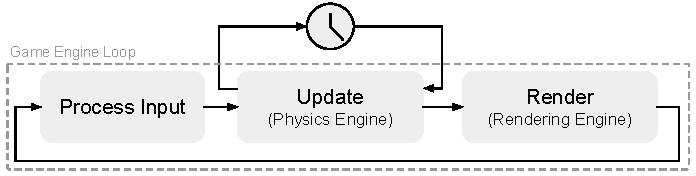
\includegraphics[width=0.5\textwidth]{Other/Figures/GameEngineLoop.pdf}
\caption{Game engine loop block diagram~\cite{GameProgPatternsBook}}
\label{GameEngineLoopDiagram}
\end{figure}

The first part of the game loop is to process the user inputs which may take the form of user keyed inputs or, in the case of AV development, the response of the AV to the current state of its environment. For example, the throttle and steering angle from the controller of an AV. The update stage interprets the input from all dynamic actors in the scene, performs any necessary physics calculations and updates the actor states. The rendering engine then takes the updated actor states and renders the scene~\cite{GameProgPatternsBook}. \todo[inline]{Fig 1: update rates of which clock?}\todo[inline]{Should there not also be a clock in the overall loop?}\todo[inline]{Greg to look up Unity wrt concurrently running processes and clocks.}

% 
% It is necessary to have an understanding of how the game loop operates in order to understand potential sources of non-determinism that are discussed below. 

As the game progresses, the game loop runs continuously according to the game clock.\todo[inline]{introduce the different clocks and what they govern, real world, game, physics and render}
%
At the beginning of each game clock tick, the lag\todo[inline]{first explain where the lag comes from} between the game clock and the real world is updated based on how much real time has passed. This measures how far the game's clock is behind compared to the real world. 
%
Then the user inputs are processed.
%
There is then an inner loop to update the physics processes (clock symbol in Fig.~\ref{GameEngineLoopDiagram}), incrementing at a delta time step, $dt$, until the game clock is equal to the real world. 
%
Rendering occurs once the game clock has caught up with the real world clock. 
%
The process then repeats.

The physics engine operates according to a time step, $dt$. %, because it makes everything simpler and more stable for physics and AI.
The shorter this time step is, the smoother the interpretation of the physical dynamics will be. %processing time it takes to catch up to game clock. % and the more deterministic the engine becomes and vice versa, as will be explained in section \ref{s:nondeterminisimSources}. 
%
Fixing the physics time step to a constant $dt$ results in simpler and more stable physics simulation and AI. 
%
To use a fixed physics time step the user's display refresh rate needs to be known in advance. This requires an update loop to take less than one render tick (one frame of real world time). Given the range of different hardware capabilities, a variable delta time is often implemented for game playing, taking the previous frame time as the next $dt$. However, variable $dt$ can lead to different outcomes in repeated tests and in some cases unrealistic physical representations~\cite{gaffer}. 
%
Semi-fixed or limited frame rates ensure $dt$ does not exceed some user-defined limit to meet a minimum standard of physical representation but allows computational headroom for slower hardware. Some engines provide sub-stepping which processes multiple physics calculations per frame at a greater CPU cost, e.g.\ Unreal Engine\footnote{\url{https://docs.unrealengine.com/en-US/Engine/Physics/Substepping/}}. 
%
If the engine tries to render between physics updates, \textit{residual lag} can occur and extrapolation between frames needs to be performed to smooth transition between scenes. This is depicted in the lower part of Fig.~\ref{GameEngineLoopDiagram}. \cite{GameEngineArchBook}\cite{GameProgPatternsBook}\todo[inline]{Should this still be cited?}\todo[inline]{Why is this part of the figure? It would be clearer if it was in a separate figure that shows all the clocks involved and how they interact - depend on each other.}
%
% Ideally the time step should be as short as possible, so that the simulation returns better accuracy of complex physical processes. %runs with high fidelity on fast machines. 
In exceptional cases where resources are scarce, the fixed time step can be greater than the time between render ticks %it takes to process an ``Update" inner loop on some (slow) machines, 
and the simulation will exhibit lag between input commands and rendered states, resulting in unsynchronised and unrealistic behaviour.\todo[inline]{Wrt the figure, is ``lag'' not a delay, i.e.\ should happen after the tick, rather than before?}

% The time step, $dt$, in the physics calculation is important and the smaller the value the more realistic the simulation will be. If $dt$ is too large or irregularly spaced then the rendered motion may not be smooth and interpolation may be required at additional computational cost. 

% This process allows hardware scalability, but the rendering will become of jerky quality on slower machines. These engines update at fixed intervals and render whenever they can, which is not steady. This results in what is so called residual lag\cite{GameEngineArchBook}\cite{GameProgPatternsBook}, where the engine is trying to render between two consecutive updates. In this case, the engine will use extrapolation techniques to give an estimate of where the object should be. This often is sufficient for gaming purposes and unnoticeable to the user, in fact it improves the stuttery motion.

\begin{figure*}[b]
    \centering
    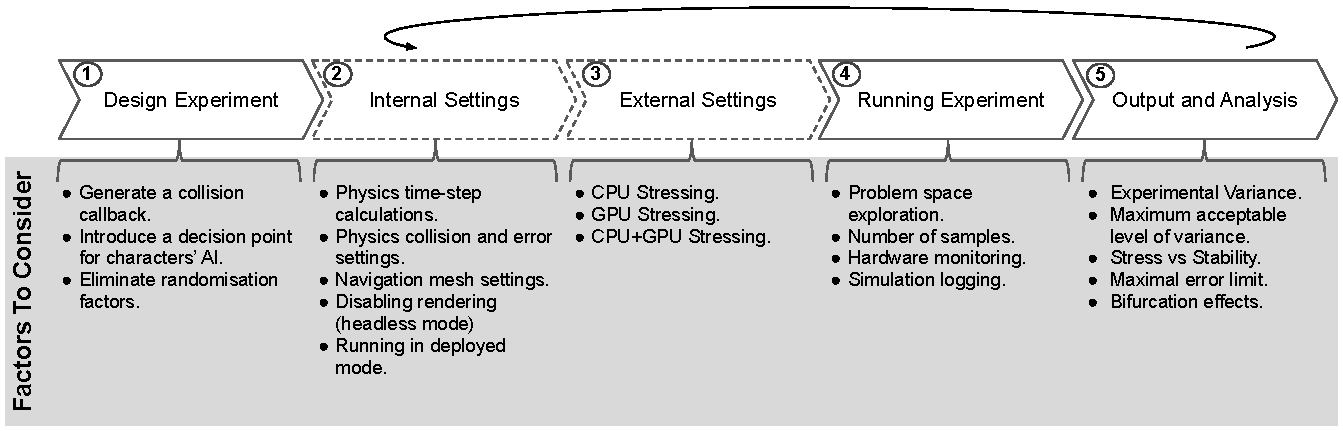
\includegraphics[width=0.99\linewidth]{Other/Figures/MethodologyDiagram.pdf}
    \caption{Flow diagram of the methodology proposed to determine the simulation variance of a simulation environment.}

    \label{method_diagram}
\end{figure*}

\todo[inline]{THIS IS IMPORTANT: Spell out the conflicting objectives (i.e.\ the fundamental differences) of gaming vs AV V\&V in terms of providing a real-time user experience at the cost of realism (for gaming) vs the need for realism potentially at the cost of losing real-time performance. This is particularly important for perception-stack testing (the sensors need to get input that is as close to the real input as possible, ideally without extrapolation or lag) and visual inspection of accidents or near misses (same is true for a human observer). For instance, see below, but I'm not sure whether this is the right place.}
In addition, providing game players with a responsive real-time experience is often achieved at the cost of realism.\todo[inline]{Do we have a ref for this, Unity vs UE4?}
%
In contrast, realism is essential in AV simulation, especially for perception stack testing, but also for visual inspection. If necessary, it is acceptable to achieve the required level of realism at the cost of the real-time user experience. 



% ======= Sources of non-determinism
\subsection{Potential Sources of Non-Determinism} \label{s:nondeterminisimSources}

The following discussion is the result of our investigation into the potential sources of non-determinism that could occur in game engines. We have examined hardware- as well as software-borne sources of non-determinism that occur at different layers of abstraction. 

\medskip

% \noindent After establishing an understanding of how physics engines work, the focus will now be on what causes these engines to be non-deterministic. The main reasons that we think are causes of these engines' non-determinism are discussed below. \\\\

\noindent\underline{\textit{Floating Point Representation:}}
Floating-point representation of real numbers is limited by the fixed bit width available in the hardware, resulting in the finite precision with which numbers can be represented in a computation. 
Thus, the results of arithmetic operations must fit into the given bit with. This is achieved through rounding to the nearest representable value, which gives rise to rounding errors~\cite{FloatingPointsBook,goldberg1991every}. 
%
% Floating-point representation of real numbers is limited with fixed register sizes resulting in errors of rounding where loss of bits occur which are rounded or truncated and cancellation which happens where two similar values are subtracted.
%
% Translating to the usage of AV simulations in physics engines,
In the context of AV simulation, this could result in precision issues of, for example, actor position within the environment leading to falsely satisfied or failed assertions.\todo[inline]{state what assertions are (used for)} 
%
One could jump to the conclusion that floating-point errors cause non-deterministic behaviour, resulting in loss of repeatability. However, these precision issues are better described as \textit{incorrectness}, rather than them being a source of non-determinism. 
%
It is safe to assume that the hardware on which game engines run is designed to be deterministic. 
%
Thus, when a rounding error occurs, then the same hardware should produce the same \textit{incorrect} result given the same operands. 
%
So, even if the result of a floating-point operation is incorrect due to floating-point rounding errors, it should always 
be equally \textit{incorrect} as long as the implementation conforms to the IEEE floating-point standard~\cite{8766229}.
%
Beyond hardware limitations, aggressive optimisations by the compiler can also introduce incorrectness in floating-point arithmetic~\cite{llvm-floating-point}. However, the same executable should still return the same output for identical input. 
%
Therefore, it can be concluded that floating point representation does not contribute to \textit{simulation variance} for repeated tests using the same executable on the same hardware.
%
% KIE: The text below is not sufficiently rigorous and not correct. 
% A generic issue with computers are floating points precision. 
%Various errors occur when doing arithmetic manipulations using floating points, especially when operating between large and small numbers due to rounding, memory limitations and so forth.\cite{FloatingPointArithmeticArticle}\cite{FloatingPointsBook}. 
%Translating to the usage of AV simulations for V\&V in physics engines, this could result in many precision issues resulting in complex non deterministic behaviours.
%
% For instance, consider a simulation where the world is infinite and progressively  generated in the physics engine. 
% After a few hundred meters, precision issues will start to occur, and will get progressively worse the further from the origin the simulation gets. 
% This is due to the values of the coordinates being used in calculations are getting bigger and hence will not cope with small values that are critical for V\&V testing purposes. 
% A solution to this problem is perhaps every time the simulations moves 100 meters away from the origin the entire world will move by 100m in the opposite direction. Thus, avoiding getting into floating point issues.\cite{FloatingPointArithmeticArticle}
%
% There are many scenarios that could be addressed, and solutions to them will entirely depend on the characteristics of that specific scenario. There is no generalised solution for the floating problem, regardless of how good computers get there will always be a limitation. However, floating points as they stand could just be sufficient for V\&V testing purposes. Whenever they are not, smart solutions can be found to accommodate for these limitations.
\\\\
\noindent\underline{\textit{Error Correcting Code (ECC) Memory:}}
ECC Memory can detect and correct single bit errors in DRAM memory. Single bit errors may occur due to malfunctioning hardware, ionising radiation (background cosmic or environmental sources) or from electromagnetic radiation~\cite{dodd2003basic}. If single bit errors go uncorrected then subsequent computational processing will produce incorrect results, potentially giving rise to non-determinism due to the probabilistic nature of such errors occurring. Estimating the rate of error is difficult and dependent on hardware, environment and computer cycles~\cite{mielke2008bit}.\todo[inline]{that said, HW simulation is deterministic, uses long simulation runs and thousands of CPU hours - I've not heard that this is an issue, but I can ask. ;)} AV verification tasks are likely to incur significant CPU hours and therefore are subject to increased exposure to these errors.
\\\\
\noindent\underline{\textit{Game Engine Code:}}
The type and version of the engine code executed should be considered, paying attention to the control of pseudo-random numbers, fixed physics calculation steps ($dt$), fixed actor navigation mesh\todo[inline]{introduce actor navigation mesh}, deterministic ego vehicle\todo[inline]{introduce ego vehicle earlier on} controllers and engine texture loading rates especially for perception stack testing. %
For example, in Unreal Editor the \textit{unit}\footnote{\url{https://docs.unrealengine.com/en-US/Engine/Performance/StatCommands/}} command can be used to determine processing bottlenecks by indicating\todo[inline]{what does indicating mean?} the total time spent generating a frame, executing the game loop or render thread.
\\\\
\noindent\underline{\textit{Scheduling:}}\todo[inline]{is this at runtime?} %
% info at:
% http://www.informit.com/articles/article.aspx?p=169479&seqNum=3
% https://www.os-book.com/OS8/os8c/slide-dir/PDF-dir/ch5.pdf
% https://en.wikipedia.org/wiki/Concurrency_(computer_science)
% https://en.wikipedia.org/wiki/Concurrent_computing
% https://en.wikipedia.org/wiki/Race_condition#cite_note-1
Scheduling is a resource management method for sharing computational resources between tasks of different or equal priority where tasks are executed dependent on the scheduler policy. A scheduler policy may be optimised in many ways such as for task throughput, deadline delivery or minimum latency~\cite{liu1973scheduling}. \todo[inline]{is this the scheduling that is done by the operating system, i.e. at runtime?}
%
If during simulation the scheduling policy was updated or thread priority was inconsistently handled, then a high variance in output may result. It is, however, unlikely that such events would occur on repeated controlled tests for the same hardware and operating system configuration.\todo[inline]{justify - WHY?}
% KIE: If all threads have the same priority, then the scheduler is free to select one, this can give rise to non-det - or not?

Similar to thread scheduling, the CPU scheduling policy determines on which processor core to execute processes in the ready queue and this is maybe ordered by factors such as throughput, latency and CPU utilisation. If the same single-threaded script executes multiple times across different physical cores due to the CPU utilisation policy then should you expect deterministic behaviour? Processor core designs should be identical although impurity inconsistency across the bulk silicon and minor perturbations in the semiconductor processing across the chip may exist. End users expect such minor variations to be controlled for in architecture tolerances and factory testing.\todo[inline]{not clear, what is the difference between scheduling cores and threads - are both done by the operating system?}

Overall, scheduling of cores or threads at runtime may be a reason for increased \textit{simulation variance}. 
%
% KIE: Not relevant here - we are just listing the sources of non-det.
% but controlling for this falls outside of the scope of this work and no attempt to control 
% these parameter have been made here. However, users should be aware of this potential issue 
% and consider methods to move towards a fixed scheduling sequence if possible.

\noindent\underline{\textit{Concurrency:}}
% Concurrency is a natural source of nondeterminism since the order and timings of independent processes can vary
\todo[inline]{Say what concurrency is and how executing concurrently running code can lead to non-determinism. Consider also parallelism, e.g. in GPUs. Focus on the order in which the execution occurs, i.e.\ the timing of events, which can cause non-determinism. Say which parts of a game engine could reasonably be expected to run concurrently.}
Another issue to consider is concurrency, where sequential tasks can be executed out of order to improve speed by utilising parallelisation depending on the decomposability of the program. This technique can lead to issues such as shared resource access conflicts and RACE conditions~\cite{huffman1954synthesis}. A game engine may use such techniques to improve performance.\todo[inline]{how?}
% KIE: We only list the potential sources of non-det, I therefore removed this. 
% although monitoring and detecting such events falls outside of the scope for this work. 

\noindent\underline{\textit{NUMA Non-Uniform Memory Access:}}
For a repeated test that operates over a number of cores based on a CPU scheduling policy, memory access time may vary depending on the memory location relative to the processor. Typically a core can access its own memory with lower latency than that of another core resulting in lower interprocessor data transfer cost~\cite{nieplocha1996global}. 
%
Changes in latency between repeated tests may, in the worst case, cause the game engine to operate non-deterministically, or, perhaps, simply with an increased data transfer cost. 
%
By binding a process to a specific core for the duration of its execution, the variations in data transfer time can be minimised.

% these may. Given the same hardware the output should always be the same, unless scheduling of the threads change. 
% i.e. the utilisation of hardware is manipulated differently each time. This would then result in non-deterministic behaviours especially if it is combined with the floating point problem discussed earlier. 
%
% For example, if a process on thread 1 requires data from thread 2, but thread 2 is delayed due to additional load then synchrony between the threads may be lost if not controlled for explicitly. Given that game engines will promote performance over accuracy the process on thread 1 may be dropped or skipped until the data are available. This may lead to events happening out of order depending on the computational load and hence non-deterministic.
%
% To solve the scheduling of threads problem, one would have to control all of the threads during runtime, which is very involved. To achieve that one would need to replace or control the whole run-time system to allocate tasks to the same threads in the same order. This is beyond the scope of our work and will not be covered in this paper.
\noindent\underline{\textit{Physics and Rendering clocks:}}
\todo[inline]{I'm not sure how VFR impacts on simulation variance, Unity claim that physics will be consistent but 'real-time' is just slowed down.}
% The inherent way of how these physics engines operate (i.e.game loops) causes the engine to be non-deterministic.  A follow up from section \ref{GameLoopSection}, these
Game engines can often have a variable game loop update rate but a fixed physics update rate, e.g.\ Unity\footnote{\url{https://docs.unity3d.com/Manual/TimeFrameManagement.html}}. This is good\todo[inline]{how?} for hardware scalability but creates a challenge for the physics calculations which provide the most consistent results with a small fixed time step. 
%
A variable frame rate\todo[inline]{Is this the game loop update rate?} could contribute to \textit{simulation variance} if the variation in the frame rate is temporally inconsistent between repeated tests and hardware.\todo[inline]{what does the hardware have to do with this? Do we not assume the same HW at this stage?} Given that variable frame rate is designed for optimising performance across differing hardware then inconsistencies across different systems may occur. Repeated tests on the same system should result in similar frame rates unless there is additional competition for resources. 
%
AV specific platforms, such as Carla, can be operated with fixed frame rates which should provide maximum stability as long as the frame rate during execution (FPS) is monitored and observed to adhere to this rate.
%
That is to say, if the frame rate is allowed to vary, then this variation has to be controlled to give the same variability throughout a given test in order for the test results to be repeatable. This issue might be of negligible significance if the frame rate is consistent and the time steps\todo[inline]{of which clock} are small enough. 

\noindent\underline{\textit{Actor Navigation:}}
Navigation meshes are used in game engines for actor path planning, and could be considered as a potential source of non-deterministic behaviour, e.g.%. Some AV simulator developers claim that the built-in physics engines' AI is non-deterministic
~\cite{CARLABenchmark}. 
This may depend on the algorithms used by the engine which typically use the A* algorithm~\cite{AStarBook} and should give deterministic outcomes as long as the environment is deterministic~\cite{AirsimUnrealArticle}\cite{UnrealAIDocumentation}. 
Therefore, the determinism of the actor path planning depends on the environment and the update to actor states within it and how navigation meshes are created or modelled, e.g. shape, granularity. 
%
It is interesting to note that changes could occur to navigation meshes if they are dynamically loaded as the simulation proceeds which can reduce computational load for large area maps\footnote{\url{https://docs.unrealengine.com/en-US/BlueprintAPI/AI/Navigation/RegisterNavigationInvoker/}}.\todo[inline]{unclear :(}
% This non-deterministic behaviour can be also resorted to the different scheduling of threads, hence giving variations in meshes every time they are loaded.

\todo[inline]{Add a summary/conclusion?}

% ***************************************************
%  METHOD
% ***************************************************
\section{Methodology} \label{s:methodology}
In this section a method for determining the variance of a simulation environment, termed \textit{simulation variance} is presented. We have identified a number of experimental parameters that may influence the simulation variance of a game engine, see Fig.~\ref{method_diagram}. These need to be considered at different stages in the process.  
%
The method requires the assessment of scenarios that exercise different actor types and functional callbacks of the game engine. These may affect different aspects of the engine as outlined in Section~\ref{s:background}, such as actor navigation and collision callbacks.
\todo[inline]{Introduce the concept of a ``callback'' as part of the background section, especially ``collision callback''.} 
%
To replicate and control the high computational loads that may be experienced in high performance simulations, software that artificially utilises resources is executed alongside the simulation on both central and graphical processing units. 
\todo[inline]{Introduce the need to use CPU and GPU HW in a game engine or any simulation HW.}
% The following section outlines a guide that may be used to determine the \textit{simulation variance} of an end user system. The aim of the experiment is to determine if the simulation is deterministic. This is achieved by monitoring actors in repeated tests and examining the deviation in path trajectories. Actors are observed in a number of different scenarios involving a mixture of vehicles and pedestrians exercising the demands outlined in Section~\ref{s:background}. 

\subsection{Setting a Determinism  Threshold}
The level of variance acceptable for a simulation must first be set. It serves as a threshold for deterministic execution.
%
We use the term \textit{determinism threshold} to refer to the acceptable level of actor path variance ($\sigma^2$), which is quoted in terms of deviation ($\sigma$) for ease of interpretation. 
%
This threshold is analogous to the analogue signal level associated with each of the binary states of the signals in digital circuits. At some low analogue voltage the signal is interpreted as binary $0$, this may be below 0.5V, and the same signal is interpreted as binary $1$ at some higher voltage, e.g.\ above 3.5V. This convention enables the abstraction from the physical signal values that are analogue voltages into the digital domain with binary representation. 

The determinism threshold depends on the objectives of the simulation and the granularity at which the simulation environment operates. In particular, this threshold must be sufficiently small to enable accurate assertion checking. \todo[inline]{Make sure assertion checking has previously been introduced.}
%


\todo[inline]{KIE: Move this to the Case Study section.}
In our case study, presented in Section~\ref{s:case-study}, a threshold must be chosen for our given application which reflects the scale at which repeatability of simulation execution is required. This value must be sufficiently small to allow accurate \textit{assertion checking} of the ego vehicle in the environment but a larger value may be acceptable for non-urban environments, e.g. motorway or highway. Similarly, the threshold value should not be so small as to fail with minor computational bottlenecks, e.g. $1\mu m$. Two autonomous vehicle projects this group are involved in, Robopilot and Capri, are looking at urban mobility and last mile delivery solutions which are predominantly concerned with urban environments rather than highway or motorway scenarios. Because of this, a deterministic threshold of $1m$ is insufficient when considering potentially dangerous close passing of cyclists and pedestrians and therefore a threshold of $1cm$ is more suitable.  

% Depending on the number of repeated tests and the average deviation reported from the experiment, a maximum rather than average may be required if the results are close to the user-specified threshold. This is to ensure that an outlier data-point is not hidden in the average of $n$-tests.

\subsection{Scenario Description}
The experiment should be a short scenario that can be easily repeated with the same initial conditions. Data logging should be used to record the actor positions at fixed time intervals throughout the simulation in order to determine the variance in actor path. The maximum deviation in actor path with respect to the mean for $n$-repeated tests will indicate at what dimensional scale deterministic results are achieved. For example, if 100 tests are executed and the maximum deviation in actor path is $<1cm$, then this scenario could be interpreted as being deterministic above this scale. 

Tests should be sufficiently repeated using statistical power~\cite{cohen2013statistical} to reveal any outlier errors that occur with low probability. Initial testing\footnote{\label{note1}Experiments using the Unreal Engine not reported here for brevity but code and experimental results can be found at \url{https://github.com/TSL-UOB/AV-Determinism/tree/master/UnrealEngineTests}} indicated an actor path deviation of $1\times10^{-13} cm$ for 997 out of 1000 tests but with 3 tests reporting a deviation of over {\raise.17ex\hbox{$\scriptstyle\sim$}}$10cm$. While executing 100 repeats may seem sufficient, in this case the sample size may fail to observe these events that occur with low probability, inferring a false confidence in the results. To ensure outlier data points are not hidden in the average of a large number of tests, the maximum deviation should be reported rather than the average when summarising.

Game engine actors can be used to simulate the AV and other vehicles and pedestrians. For the experiment, actors should follow a series of trajectory waypoints which are hard-coded for each test type. In our experiments, hard-coded target location goals regularly spaced at $1m$ intervals were used for pedestrians and vehicles ensuring all actors were given the same initial conditions and any variation comes from execution of the simulator at runtime. Initial testing also indicated that when actors collide there is a significant change in \textit{simulation variance}, therefore the experiment should include some scenarios where collision callbacks are activated. 

It is also important to control any pseudo-random numbers that are called in any external during the simulation with fixed seeds to ensure repeatable testing, e.g. external vehicle control programs or other clients connected to the simulator. 


% \todo[inline]{Abanoub: what is the distance between your hard-coded waypoints, are they regularly spaced? Might need to talk about interpolation code and give link to github}

% \todo[inline]{In our experiment, gross waypoints were interpolated to give a regularly spaced set of coordinates approximately $1m$ apart, and this interpolated set of waypoints were used as "target location goals" (AB: not sure what the correct terminology is here) for the pedestrian actors. %
% For the vehicles in the simulation, waypoints are generated and interpolated in the same way but execution at runtime is slightly different where a PID controller is used to generate a velocity profile and steering angle requests to reach the destination targets.}

% We use game engine actors to simulate the AVs and other agents (vehicles and pedestrians). Actors can either follow a series of trajectory waypoints or can plan a route to a further destination using some path planning and obstacle avoidance algorithms, e.g. A* search algorithm. 
 
\subsection{System Resources}
To simulate the demands of taxing simulations, potentially requiring realistic rendering or complex physics calculations in an otherwise simple scenario, stress programs should be used to artificially occupy system resources. Preliminary work\footnote{see footnote 14} suggested that adding stress to the CPU or GPU will  contribute towards increased \textit{simulation variance}. CPU utilisation software, such as the linux \texttt{stress} tool which is a workload generator program that can be used spawn workers on any number of cores or virtual threads on a system. This can be used to artificially increased the load on the system to explore at what point your system may become unstable leading to \textit{simulation variance}. For GPU utilisation \texttt{gpu-burn} was employed using the fur test at different resolutions and multiple instances can be used to generate high utilisation levels~\cite{GPU_stress}.

% The user should also monitor and record system CPU and GPU utilisation rates. Additionally, if the user is interested in real-time assessment of the simulation then FPS should also be monitored and logged.

% Collision callbacks
% \subsection{Other Considerations}
% \noindent When designing the experiment(s) one needs to bare in mind the following two questions: i) Is the engine deterministic? ii) If not, how does its simulation variance vary? In simulation, actors can either follow a series of trajectory way points or they get given the destination and their AI path plans to that destination. Thus, given that an engine has a high level of simulation variance, then one needs to set up an experiment that would stress the engine in order to determine how its simulation variance vary. 
% This is best done by generating collision callbacks, because that is when engines' do a lot of calculations to determine the response after the collision. Another approach, if AI is used for path planning instead of just following predefined trajectory way points, is to introduce a decision point for the AI.\\\\
% The user should set a deviation threshold, beyond which simulation results deemed unacceptable or non-deterministic. For the majority of AV navigation on major roads and highways a limit of $1m$ may be acceptable but in denser urban environments a value of $1cm$ may be more appropriate. 


\subsection{Internal settings}
Where possible a fixed $dt$ should be used to give the most reliable physics calculations. If using Carla a small fixed value, say $0.05s$, can be set by using the following: \texttt{setting.fixed\_delta\_seconds = 0.05}, whereas in Unity the default fixed time step is set to $0.02s$\footnote{\url{https://docs.unity3d.com/ScriptReference/MonoBehaviour.FixedUpdate.html}} and a good description of the interplay between physics and render clock is given here~\cite{JohnAustinUnity}. In Carla, further settings can be applied to allow synchronous communication to external controllers to ensure no sensor data are passed out of order to the simulator~\cite{carla_sim_config}.

Within Unreal Engine there are numerous internal settings relating to the movement and interaction of physical bodies in the simulation. Settings can be adjusted to alter how actors interact and path plan via the navigation mesh of the environment, e.g. \textit{Contact Offset} and \textit{Navmesh Voxel Size}, or can be changed to improve the fidelity of physics calculations between game update steps, e.g. \textit{Physics Sub-Stepping} and \textit{Max Physics Delta Time}. Other options such as \textit{Enable Enhanced Determinism} were investigated along with running the engine from the command line with options for more deterministic behaviour \texttt{-deterministic}, floating point control \texttt{/fp:strict} and headless mode \texttt{-nullrhi} along with running the test as a packaged release by building and cooking\footnote{\url{https://docs.unrealengine.com/en-US/Engine/Deployment/Releasing/}}. However, none of these options improved simulation variance significantly beyond the default settings, see our previous investigation~\cite{TSLUnrealEngineTesting}.

% By doing various inspections around them we did not notice much improvement or worsening in the simulation variance between test runs, therefore the internal settings option was disregarded. However, one of the options we used is synchronous mode with a fixed time step that is available in CARLA. This would make the simulator proceed to the next tick only when commanded to do so by our script, which makes runs' flow more consistently.  

% There are several error and physics collision internal settings in physics engines that can be tweaked to enhance the simulation variance of the engine.
% Increasing the physics time-step calculations, which is increasing the number of calculations per unit time, would improve the simulation variance since the physics sequence will be more finely defined; but on the other hand this would be more computationally expensive. However, in such applications of V\&V of AV simulations, the computational cost should be of less concern compared to the importance of repeatability of tests.
% If the experiment setup includes the usage of the physics engine's AI then altering the navigation mesh settings in the engine, like increasing the granularity of the mesh or changing the mesh type; can improve the simulation variance as a result of allowing the AI to navigate in a more well defined space. 
% Disabling rendering or running in headless mode is a way of attempting to entirely decouple the rendering engine from the physics engine, which theoretically should affect positively the repeatablility of tests. 
% The downside of most physics engines is that they do not provide a headless mode in the editor setup, thus this could make running in headless mode a real challenge for verification engineers.
% Running in editor or deployed mode can sometimes cause differences in performance, with deployed mode being worse, mostly due to the way settings get packaged when in deployed mode.

% \begin{table*}[b]
% \centering
% \begin{tabular}{clclcc}
% \toprule
% Test ID & Test description (See Figures~\ref{Test_a} and \ref{Test_b}) & Collision/Intersection & Collision Type & Look ahead distance (m) & No. of repeats \\ \midrule
% 1       & Two vehicles driving                   & No  & N/A & 2 & 1000 \\
% 2       & Two vehicles driving                   & Yes & Vehicle and Vehicle & 2 & 1000 \\
% 3       & Two vehicles driving and a pedestrian  & No  & N/A & 2 & 1000 \\
% 4       & Two vehicles driving and a pedestrian  & Yes & Vehicle and Pedestrian & 2 & 1000 \\
% 5       & Two pedestrians                        & No  & N/A & 2 & 1000 \\
% 6       & Two pedestrians                        & Yes & Pedestrian and Pedestrian & 0.4 & 1000 \\
% 7       & Two pedestrians                        & Yes & Pedestrian and Pedestrian & 2 & 1000 \\
% 8       & Two pedestrians                        & Yes & Pedestrian and Pedestrian & 20 & 1000 \\
% \bottomrule
% \end{tabular}
% \caption{Set of experiments}
% \label{TableOfExperiments}
% \end{table*}

\begin{table*}[b]
\centering
\begin{tabular}{clclccc}
\toprule
Test & Actors 					 	  & Collision 	 & Collision Type 			 & $n$  & $\max\sigma$ (m) & $\max\sigma$ (m) \\ 
	 & 								  & 			 & 							 &	    & (unrestricted)  & (restricted)	\\ \midrule
1    & Two vehicles                   & No  		 & N/A 			  			 & 1000 & 0.03 & $7.0{\times}10^{-3}$ \\
2    & Two vehicles                   & Yes 		 & Vehicle and Vehicle 		 & 1000 & 0.31 & $9.8{\times}10^{-3}$ \\
3    & Two vehicles and a pedestrian  & No  		 & N/A 			  			 & 1000 & 0.07 & $5.2{\times}10^{-4}$ \\
4    & Two vehicles and a pedestrian  & Yes 		 & Vehicle and Pedestrian 	 & 1000 & 0.59 & $1.5{\times}10^{-12}$ \\
5    & Two pedestrians                & No  		 & N/A 			  			 & 1000 & $5.6{\times}10^{-13}$ & $5.6{\times}10^{-13}$ \\
6    & Two pedestrians                & Yes 		 & Pedestrian and Pedestrian & 1000 & $5.6{\times}10^{-13}$ & $5.6{\times}10^{-13}$ \\
\bottomrule
\end{tabular}
\caption{A description of the test scenarios showing the test number, the actors included and if a collision occurred and between which actors. Where $n$ is the number of repeats and $\max\sigma$ is the maximum simulation deviation. The term \textit{unrestricted} refers to an unrestricted subset of the results and allowing system states of any resource utilisation whereas \textit{restricted} employs results filtering to pre-collision and limits system resource utilisation levels to 75\%.}
\label{TableOfExperiments}
\end{table*}

% \subsection{External settings}
% Running other programs in the background, like having a web browser open, or running the physics engine in the background while performing other tasks on the same machine does also have an effect; because it alters the CPU and GPU utilisation of tasks. Trying to run stress experiments on computers by running other programs makes it difficult to control experiments since the utilisation would be inconsistent, nonetheless, there exists dedicated stress utilisation programs which provide consistent CPU and GPU stressing. Note that during running these tests computers should be left alone and not to be used for any other purposes apart from running the experiments, else the CPU + GPU stressing will lose its consistency through out a given test. 

% \subsection{Running experiment}
% \noindent When it comes to running the experiment itself, things that one should consider are the problem space exploration; the number of runs that should be executed to get reliable results; the frequency of logging data of actors; and possibly having a program to monitor the hardware utilisation.
% Problem exploration, there is too many variables that one can play with. do statistical analysis some.... some of them get problematic...

\subsection{Output and Analysis}
The output for each experiment can be summarised as the \textit{maximum variance} of any actor over the $n-$repeated tests. The maximum variance is chosen to indicate the worst case rather than an average which could hide outlier data points when a high number of repeated tests are performed. This value can be analysed against the different scenarios or settings that have been identified as potential sources of simulation variance. These values can then be assessed against the user-defined \textit{deterministic threshold} to determine if the simulation is deterministic or not. 

% Once the experiments are run, the logged data is post processed to find the variance in the logged data between the different runs. Note that bifurcation effects can cause a jump in the variance, so it is worth plotting the different logged paths in order to determine if there are any bifurcation effects.

% This whole process is repeated for various internal and external settings (if needed). 
% Then various plots can be created to draw the engine's simulation variance. 
% Thereon, it would be up to the verification engineers to determine where they want to define the line below which the simulation variance would be acceptable, and thus know at which levels of computational utilisation they can guarantee to run repeatable experiments.   


% ***************************************************
%  CASE STUDY
% ***************************************************
\section{Case Study} \label{s:case-study}
We present a case study to illustrate some the challenges of simulation based verification outlined in Section~\ref{s:introduction}. The simulation must be deterministic and by our definition this should mean that the overall level of simulation variance $\sigma^2$ for any actor should be less than a user-defined threshold. Results are shown in terms of the maximum deviation ($\sigma$) and the deviation threshold in our case is $1cm$, where any value higher than this is considered non-deterministic. 

In order to reproduce conditions for computationally intensive simulations, the experiments are executed with additional levels of artificial resource utilisation. Resource utilisation was artificially increased for both CPU and GPU devices (see Section \ref{s:methodology}) using reported values of the system monitors \texttt{htop} and \texttt{nvidia-smi} respectively. Resource utilisation figures reported here should be considered approximate values.
% The level of additional resource utilisation, above that of the needs of the simulation, was increased from $0\%$ (no additional resource load) in $25\%$ increments up to a maximum of $95\%$ for both CPU and GPU as reported by system monitors (\texttt{htop} and \texttt{nvidia-smi} respectively). 

\subsection{System Configuration and Screening}
These tests were carried out on an Alienware Area 51 R5 with an i9 9960X processor with 64GB DDR4 RAM at 2933MHz with an NVIDIA GeForce RTX 2080 graphics card with 8GB GDDR6 RAM at 1515 MHz. To ensure reliability of results, each test was repeated 1000 times. Tests were carried out in Carla using synchronous mode with a fixed $dt$ of $0.05s$. To ensure our experiment did not fall foul of some of the possible sources of non-determinism outlined in Section~\ref{s:nondeterminisimSources} a series of screening tests were performed on our system. These were:

\begin{itemize}[leftmargin=*]
    \item System memory: \texttt{memtest86}\footnote{\url{https://www.memtest86.com/}} full suite of tests ran, all passed.
    \item Graphical memory: \texttt{cuda\_memtest}\footnote{see \url{https://github.com/ComputationalRadiationPhysics/cuda_memtest}} full details of tests found here~\cite{shi2009testing}, all tests passed.
    \item Non-uniform memory access: \texttt{numactl}\footnote{\url{https://linux.die.net/man/8/numactl}} was used to fix the simulator and test script to single cores but only a minor (2\%) improvement in simulation variance was observed and therefore not used for subsequent testing.
\end{itemize}

% Given that our interest is on AV simulations, this study presents a number of experiments run on typical agents used in AV simulations and their interactions with each other. These agents are classified into two, either vehicles(cars, motorcycles, bikes etc.) or pedestrians (can include animals). Here we will walk through our hypothesis, description of our tests and the analysis of results from the different tests. We will point out at each stage where we sit in Figure~\ref{method_diagram} as we go through this case study.    

% \subsection{Problem And Hypothesis}
% We want to see whether using Unreal Engine 4 (UE4) along with CARLA \cite{CARLA_paper} for V\&V of AV simulations is deterministic or not; if not then what is the simulation variance that we will operate with, is it acceptable or not, and whether it worsens with stressing GPU and CPU.

% Our hypothesis is that since UE4 is a game engine it is not deterministic, however, the simulation variance would be very low to acceptable limits that allows verification engineers to use it confidently and assume that tests would be repeatable. This behaviour is expected not to hold as the level of computing stress increases.     

% \subsection{Tests Description And Technicalities}\label{TestsDescriptionAndTechnicalities}
\subsection{Scenario Description}\label{TestsDescriptionAndTechnicalities}
The list of tests shown in Table \ref{TableOfExperiments} were chosen to cover a range of interactions between actor types. Tests 1 \& 2 involve 2 vehicles meeting at a junction where they do not collide (test 1) and when they do tiggering a collision callback in the game engine (test 2). In both cases the trajectories of the vehicles are hard-coded to follow a set of waypoints spaced at $0.1m$ intervals using a PID controller. In test 3 a mixture of different actor types are introduced where two vehicles dive without collision and a pedestrian walks across the road at a crossing point. In test 4 this pedestrian collides with one of the vehicles at the crossing triggering a collision callback, see Fig~\ref{Test_a}. Similar to vehicles, pedestrians navigate via a set of regularly space waypoints at $0.1m$ intervals using the A* algorithm which is the default controller for the Carla pedestrian actors. Tests 5 \& 6 involve only pedestrians where they do not collide (test 5) and where they do (test 6), see Fig.~\ref{Test_b}. 

 % targetting the closest waypoint but ignoring any waypoints closer than a fixed \textit{look-ahead distance} ($d_l$)\footnote{Targeting waypoints with $d_l<0.4$ tend to cause improper navigation with the implemented PID controller}.
% Pedestrians have the functionality of dynamic path planning i.e. they can avoid obstacles to reach their waypoints and so they can avoid static objects and other actors. To ensure they intersect (collide) with each other $d_l$ is altered; the smaller the look ahead distance the less chance the pedestrian will get to path plan around each other, and thus making sure they intersect. (This sounds like at some $d_l$ the pedestrians do not collide - is this true?) 


% Similar to the vehicle actors, the look ahead range ($d_l$) can be modified so that the actor is forced to navigate on waypoints that are further away. In test 7 $d_l$ is increased from $0.4m$ to $2.0m$ and in test 8 to $20m$ which was done to investigate if the path planning algorithm was deterministic when given waypoints further ahead.

% The vehicles in this simulator follow a trajectory of waypoints using a PID controller and they have a look ahead distance that they target for from a given list of trajectory waypoints. Similarly with the pedestrians, but they don't have a PID controller and they can do dynamic path planning using A* algorithm to reach their destination or in this case a trajectory waypoint.

% Starting from step 1 in the methodology diagram (Design Experiment); we are using a double mini roundabout for our experiments. 

% The list of tests shown in Table \ref{TableOfExperiments} were chosen to cover the mandatory interactions between the different types of agents. These are summed up in the following: \textbf{i)}Agents (vehicles and pedestrians) moving with no collisions or interactions with each other \textbf{ii)}Collision between vehicles \textbf{iii)}Collision (intersection) between pedestrians \textbf{iv)}Collision between vehicles and pedestrians.


\begin{figure}[!t]
    \centering
    \begin{subfigure}{.24\textwidth}
        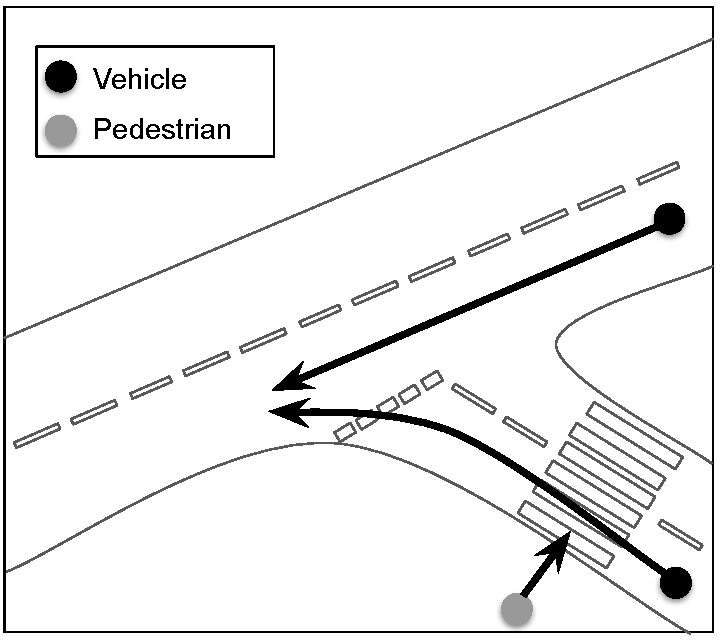
\includegraphics[width=1\textwidth]{Other/Figures/TestCasesDiagramV2_a.pdf}
        \caption{}
        \label{Test_a}
    \end{subfigure}
    \begin{subfigure}{.24\textwidth}
        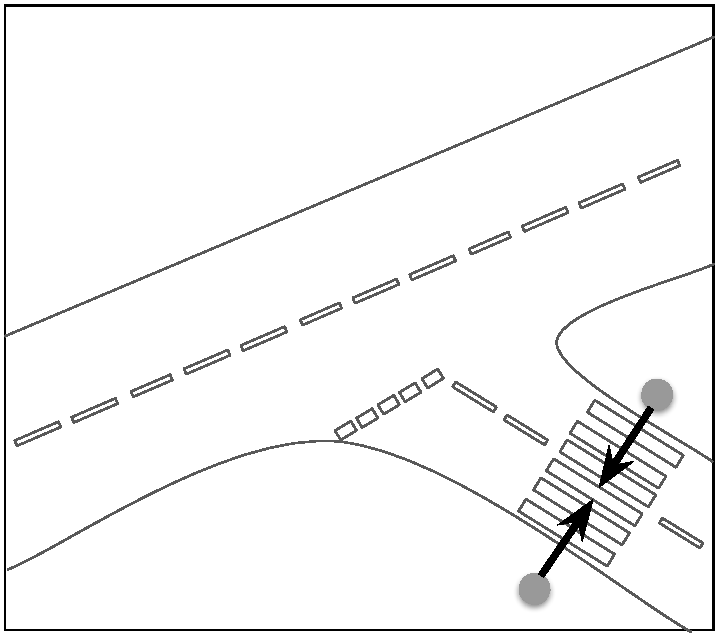
\includegraphics[width=1\textwidth]{Other/Figures/TestCasesDiagramV2_b.pdf}
        \caption{}
        \label{Test_b}
    \end{subfigure}
    \caption{Schematic of test scenarios for (a) tests 1-4, (b) tests 5-6. Descriptions are given in Table~\ref{TableOfExperiments}.}
\end{figure}

\begin{figure}[!t]
    \centering
    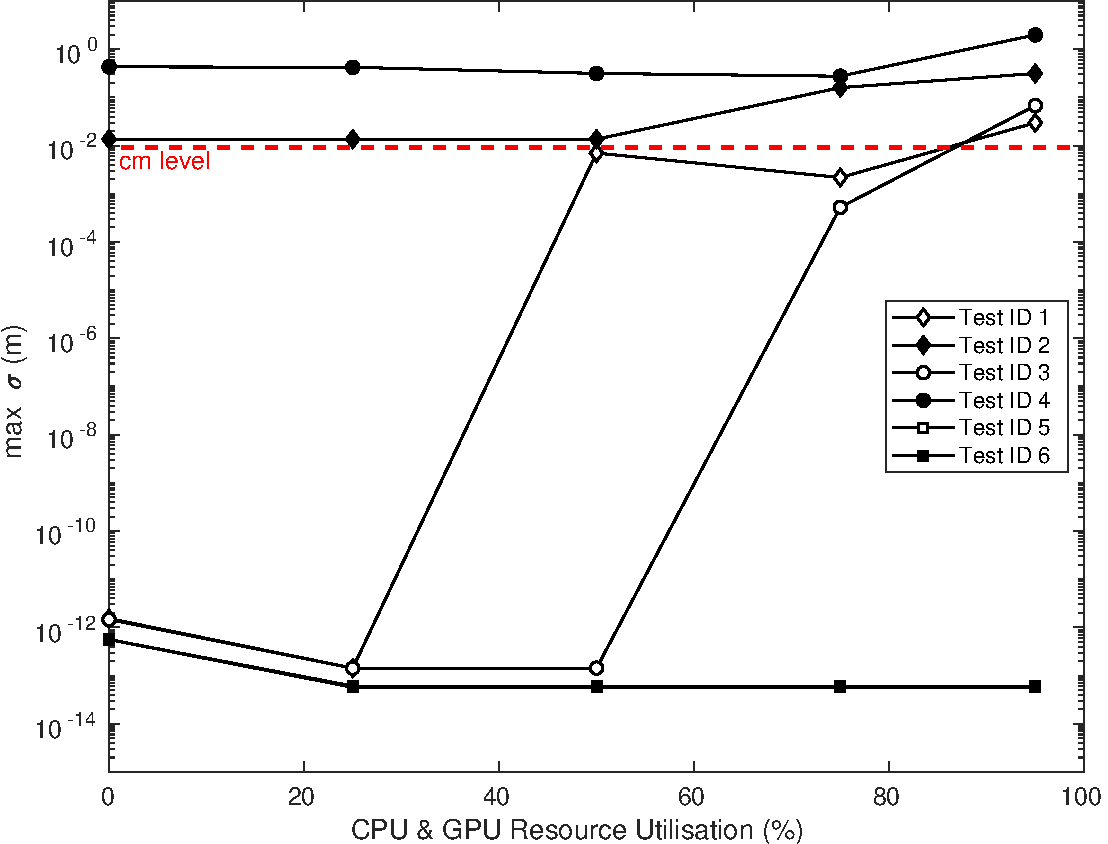
\includegraphics[width=0.48\textwidth]{Other/Figures/ExperimentsStressSummaryV4.pdf}
    \caption{Summary of results showing maximum deviation for each scenario against different resource utilisation levels. Tests 5 and 6 overlap having almost identical results.}
    \label{ExperimentsStressSummary}
\end{figure}

% Tests 1, 3and 5 are similar and there are no collisions in them, they were done as separate tests (instead of combining them into one) for the sake of simplicity and to use them as base lines for the tests-collision versions of them. The tests for collisions and non-collisions differ by a very slight change in the trajectory of the agents just to make them avoid colliding or intersecting with each other.

% Test 2 is a collision between two vehicles and no pedestrians involved and is depicted by \ref{Test_a}, where the two vehicles will approach the roundabout and crash.

% Tests 6,7 and 8 are tests with pedetrians having the same trajectory waypoints but walking in opposite directions to each other (see Figure~\ref{Test_b}). 
% Pedestrians have the functionality of dynamic path planning i.e. they can avoid obstacles to reach their waypoints and so they can avoid bumping into each other. Hence, to make sure they intersect (collide) with each other then we  have set tests 6,7 and 8 to be the same but with different look ahead distances; the smaller the look ahead distance the less chance they will get to path plan around each other, and thus making sure they intersect.

% In V\&V of AV simulations, collisions of pedestrians together is not of much interest, nevertheless we decided to include these tests for the sake of completeness and to obtain a full image of the simulation variance of the simulator.

% Test 4, is where a vehicle hits a pedestrian and runs over it on a zebra line, as shown in Figure~\ref{Test_a}.

% Proceeding to step 2; there is about 20 different internal settings related to our context that can be tweaked in UE4; such as \textit{Enable Enhanced Determinsim}, \textit{PhysX Tree Rebuild}, \textit{Max Physics Delta Time} etc. By doing various inspections around them we did not notice much improvement or worsening in the simulation variance between test runs, therefore the internal settings option was disregarded. However, one of the options we used is synchronus mode with a fixed time step that is available in CARLA. This would make the simulator proceed to the next tick only when commanded to do so by our script, which makes runs' flow more consistently.  

% On the other hand the external settings (step 3), where CPU + GPU are stressed, did show significant variations in the results as will be discussed in section \ref{ResultsSection}. Different levels of stress were applied to the computer; using the \texttt{stress} function \cite{CPU_stress} to stress the CPU and \texttt{gpu-burn} from github \cite{GPU_stress} to stress the GPU.

% In terms of running the experiments (step 4), \textbf{i)} the computer used is an Alienware Area 51 R5 with an i9 9960X CPU chip, NVIDIA GeForce RTX 2080 graphics card and 64GB of RAM; \textbf{ii)} \texttt{nvidia-smi} and \texttt{htop} were used to monitor the levels of GPU and CPU stress respectively before and while the experiments were executed \cite{monitoring_stresses}; \textbf{iii)} the computer was left alone and not used for any other tasks while the runs were executed.

% ***************************************************
%  RESULTS
% ***************************************************
\subsection{Results And Discussion}\label{ResultsSection}
The summary of all the tests are shown in the final column of Table~\ref{TableOfExperiments} where $\max\sigma$ is the maximum deviation across all resource utilisation levels. From these summary results it is clear that scenarios with only pedestrian actors are those that are consistently deterministic over all resource utilisation levels. However, for other scenarios involving vehicles or a mixture of actors types resource utilisation level has a significant impact on \textit{simulation variance}.

Figure~\ref{ExperimentsStressSummary} shows $\max\sigma$ against resource utilisation level, where the $x$-axis indicates the approximate percentage of resource utilisation (CPU \& GPU). In this figure, anything above the $cm$ threshold (dashed line) is considered non-deterministic according to our specific threshold level informed from our verification requirements. A general pattern in the results indicates that some scenarios fail to produce deterministic results consistently against any resource utilisation level and that some cases only fail at utilisation levels above 50\%.

However, the non-deterministic results in Figure~\ref{ExperimentsStressSummary} (all those above the dashed line) are the worst case account of the situation. Examining these specific results, tests 2 \& 4, in more detail as a function of simulation time reveals further information about the simulation variance before and after an actor collision. Fig.~\ref{CarsCollisionCG25} shows this examination for vehicle to vehicle collisions (test 2), where $\max\sigma$ switches from deterministic prior to the vehicle collision and is non-deterministic post-collision. This pattern of deterministic behaviour prior to collision is maintained up to a resource utilisation level of approximately 75\%, Fig.~\ref{CarsCollisionPrePost}. This time series examination was repeated for vehicle to pedestrian collisions (test 4) and the results are shown in Fig.~\ref{CarsPeopleCollsionsCG25}. Similarly to vehicle collisions, the variation of $\max\sigma$ for vehicle to pedestrian collisions indicates pre-collision deterministic behaviour with up to 75\% resource utilisation, Fig.~\ref{CarsPeopleCollisionPrePost}. This is a key finding of this work and suggests that verification engineers should consider this as an end condition for terminating tests as any post-collision results are not reliable. 

The second key finding of this work is illustrated in Fig.~\ref{CarsPeopleCollsionsCG25}. In this scenario (test 4), there is a collision between Car ID 2 (solid line) and Ped ID 3 (dot dash line) which occurs at a simulation time of approximately $6s$ and the other vehicle, Car ID 1, is \textit{not involved in the collision}. There are three key observations here; firstly that the vehicle directly involved in the collision (Car ID 2) displays non-deterministic actor position post-collision as describe above. Secondly, that the pedestrian involved in the collision (Ped ID 3) displays deterministic behaviour throughout the test\footnote{note that in Carla the pedestrian object is destroyed post-collision hence the flat line following the collision}. And, thirdly we observed a delayed effect on Car ID 1 showing high simulation variance with a $5s$ delayed effect \textit{even though this vehicle was not involved in the collision}. This final point should be of particular concern to verification engineers and research practitioners in the field as it implies that any collision between actors will affect the simulation variance of all actors in the simulation and could potentially result in false-positive assertion violations.

% \textbf{Strange gap post-collision for few seconds}

% \textbf{Should we rename 'test' to 'scenario???'}

\textbf{Big question why does high-RU influence simulation variance?? Can we tie this to thread scheduling and will NUMAclt change this conclusion?'}

% Scenarios that include both collisions and vehicle actors were not deterministic. However, when observing the deviation in actor paths against simulation time, Fig.~\ref{CarsCollisionCG25}, the simulation is deterministic prior to collision but not afterwards. 

% This was calculated by averaging the variance between all of the different runs through out the simulation time for all of the agents, then taking the square root to obtain the total mean devaiton. Note the dotted red line in the plot shows the millimeter (mm) level. Below this level we assume that the simulation variance is low enough that it would not affect our assertion checking for V\&V of AV simulations purposes, that it is sufficient to assume the tests are deterministic and repeatable. This line can be moved up or down and it is entirely up to verification engineers where they want to define the level below which tests' variance is negligibale and it is suffcient to assume that tests are deterministic.



\begin{figure*}[h]
    \centering
    \begin{subfigure}{.49\textwidth}
        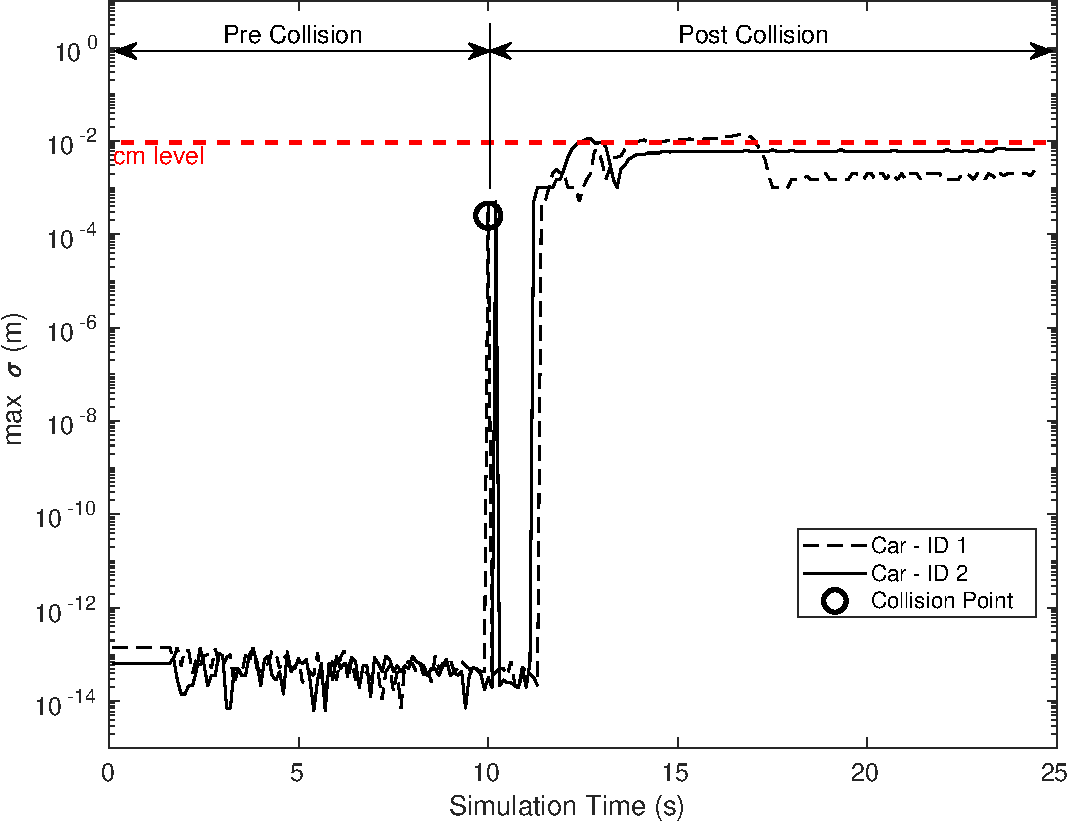
\includegraphics[width=1\textwidth]{Other/Figures/CarsCollisionCG25_V3.pdf}
        \caption{}
        \label{CarsCollisionCG25}
    \end{subfigure}
    \begin{subfigure}{.49\textwidth}
        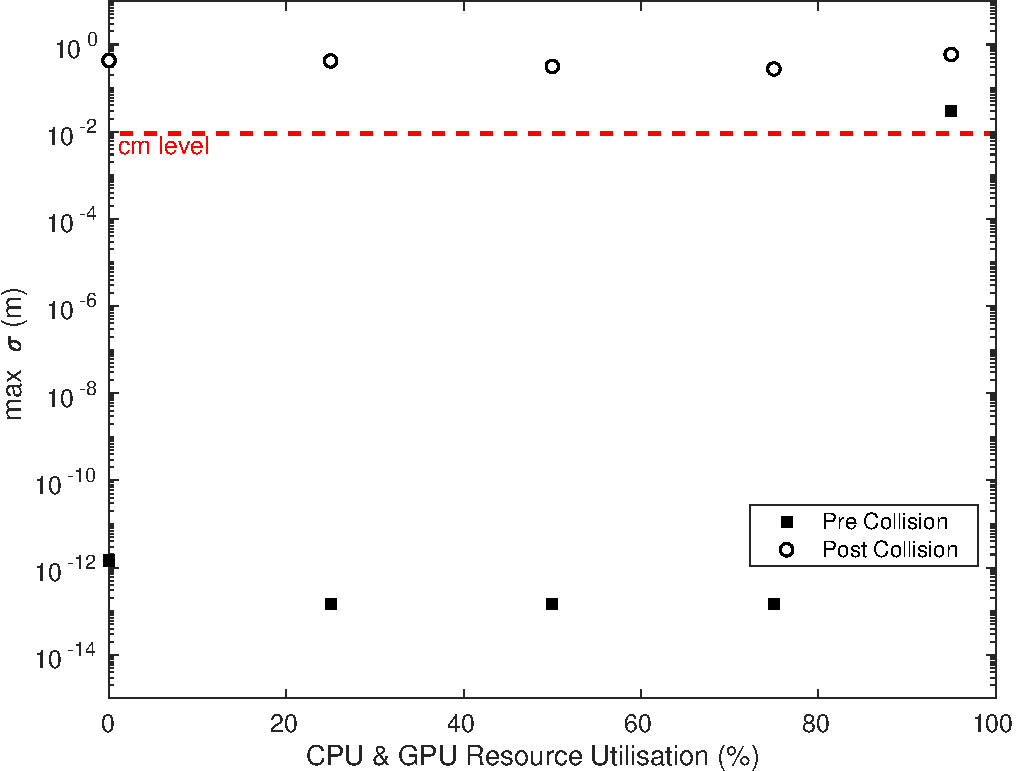
\includegraphics[width=1\textwidth]{Other/Figures/CarsCollisionPrePostV3.pdf}
        \caption{}
        \label{CarsCollisionPrePost}
    \end{subfigure}
    \caption{Vehicle to vehicle collision (test 2) showing (a) mean deviation against simulation time for 25\% resource utilisation and (b) mean deviation pre- and post-collision against resource utilisation.}
\end{figure*}

\begin{figure*}[h]
    \centering
    \begin{subfigure}{.49\textwidth}
        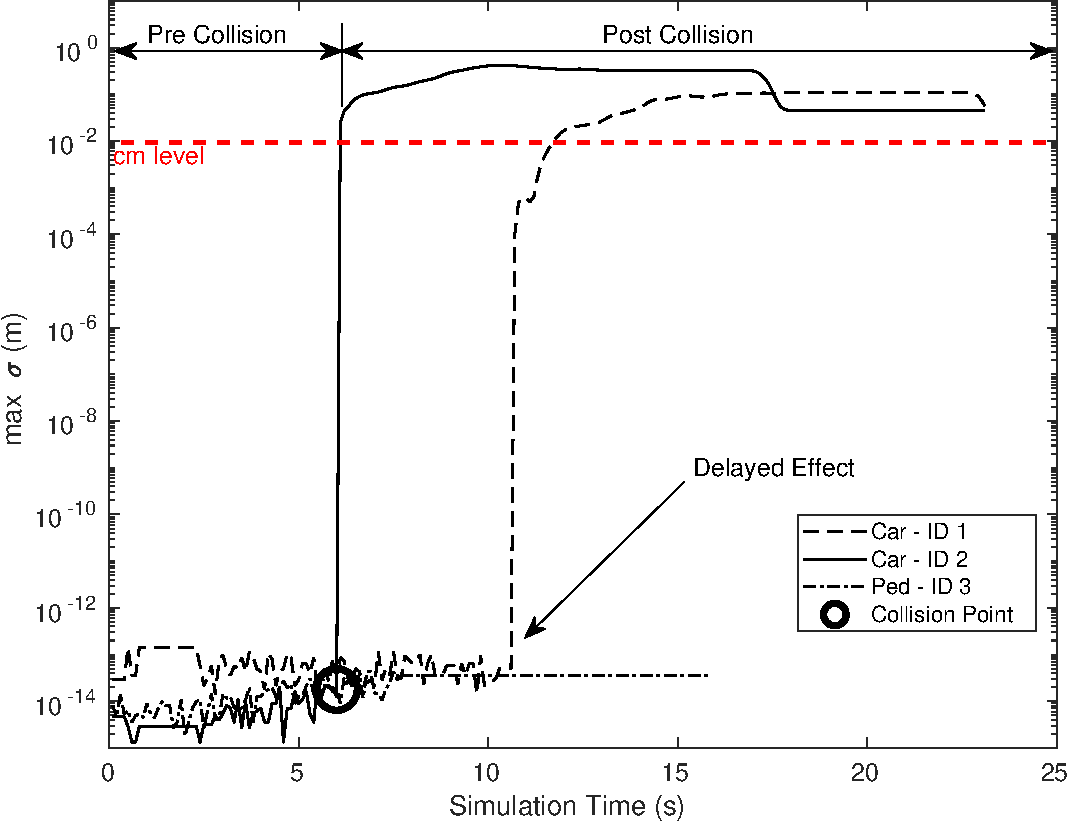
\includegraphics[width=1\textwidth]{Other/Figures/CarsPeopleCollsionsCG25_V3.pdf}
        \caption{}
        \label{CarsPeopleCollsionsCG25}
    \end{subfigure}
    \begin{subfigure}{.49\textwidth}
        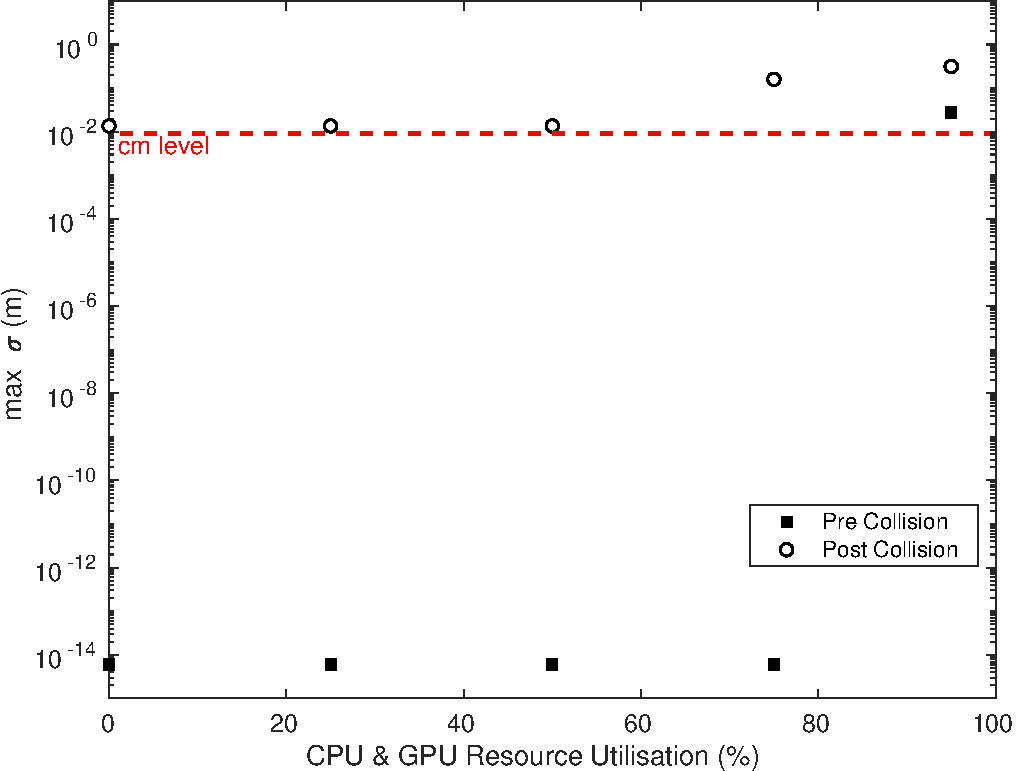
\includegraphics[width=1\textwidth]{Other/Figures/CarsPeopleCollisionPrePostV3.pdf}
        \caption{}
        \label{CarsPeopleCollisionPrePost}
    \end{subfigure}
    \caption{Vehicle to pedestrian collision (test 4) showing (a) mean deviation against simulation time for 25\% stress and (b) mean deviation pre- and post-collision for different resource utilisation.}
\end{figure*}

% First, the tests with no collisions are considered, these represent tests 1, 3 and 5. Tests 1 and 3, which involves vehicles only and vehicles with pedestrians respectively, shows very low simulation variance for stress levels below 50\% and as the stress level increases they surpass the red line crossing our defined deterministic level but still being sufficiently low (i.e. with in the centimeter level). This clearly shows how the load on a computer (i.e. stressing CPU and GPU) can have drastic effects on the repeatablitiy of tests. This is more specific to vehicle agents rather than pedestrians since the behaviour of pedestrians is consistent and remarkably below the mm level for all of the different levels of stress shown by test 5, where only pedestrians are involved with no collisions, from which it can be deduced that the mean deviation change with the stress level in test 3 was solely due to the vehicles.

% Next, given the pedestrians were showing low simulation variance, we ran tests for pedestrians colliding (i.e. with paths intersection) for different look ahead distances to exploit whether that would cause any changes, but yet as it can be seen by lines Test IDs' 6,7 and 8 that their performance is consistent for all of the different tests.

% Finally, we look at the other collisions tests, tests 2 and 4 where the tests correspond to a collision between two vehicles and a collision between a vehicle and a pedestrian respectively. We observe that in both of these tests the mean deviation is always above our red line regardless of the stress level, nevertheless still increasing the stress levels shows worsening effects.

% Thus, we resorted to plotting the mean deviation over the number of runs of these two tests vs simulation time with stress level \%25 chosen arbitrarily (see Figure~\ref{CarsCollisionCG25} and \ref{CarsPeopleCollsionsCG25}). Doing that we discovered that after collisions occur there is a jump in the mean deviation, which is what causes the averaged mean deviation through the whole simulation time in Figure~\ref{ExperimentsStressSummary} to always surpass our red line.

% Plotting Figures~\ref{CarsCollisionPrePost} and \ref{CarsPeopleCollisionPrePost}, which shows the mean deviation pre and post collision for the different stress levels; it can be seen that there is two discrete levels for the pre and post collison devaition from these plots and as the stress increases these two discrete levels start to merge. However, in V\&V of AV simualtions we  are normally interested in the point until a collision occur after which the simulation will be terminated. Thus, the post collision effect should not be of much concern in the context of AVs. 

% It is important to note, however, that in test 4 a delayed effect of increase in simulation variance was noticed to Car ID 1, which interestingly was not involved in the collision, this was attributed to how the physics engine was programmed to calculate collisions which might cause other obscure behaviours to other agents. The importance of this outcome is that it shows even if an ego vehicle is not involved in a collision, but other agents are, this will still have effects on the simulation variance of the ego vehicle. Thus failing to stay below our red line and the test should be terminated. In summary, from the tests carried out we can deduce that for a computer of the following specifications, an Alienware Area 51 R5 with an i9 9960X CPU chip, NVIDIA GeForce RTX 2080 graphics card and 64GB of RAM, that all tests carried out using CARLA in UE4 are gauranteed to be deterministic and repeatable (according to our definition by the red line) as long as the CPU + GPU stress does not exceed 50\% and tests are terminated as soon as a collision of any type is detected in the simulation. 

% ***************************************************
%  CONCLUSION
% ***************************************************
\section{Conclusions}\label{s:conclusion}
Practitioners in this field can resolve the non-deterministic operational domains of their simulation by following the method outlined in this paper. Potential sources of non-deterministic simulation behaviour have been discussed such as floating point rounding error and scheduling policy. A case study was used to ascertain the boundary between deterministic and non-deterministic operation of the Carla driving simulator. Results suggest non-deterministic outcomes when resource utilisation levels exceeded 75\% or when vehicle collisions occur for the particular hardware used in this study. Furthermore it was found that all actors, even those not involved directly in a collision, will behave non-deterministically if a collision callback to the game engine is made. Best operating practice follows that the simulation should be stopped as soon as a collision callback is detected or resource utilisation levels exceed 75\% although this value may be system specific. 

% We have provided a summary of the sources of non-determinisim in game engines. This was followed by presenting a method by which one can determine the simulation variance of a game engine used in V\&V application of AV simulations. The method consists of five stages, starting with designing the experiment, then suggesting the various settings that can improve or worsen the performance, and finally focuses on running the experiment and analysing the output.

% A case study is then used to show the implementation of the method introduced, where several tests were setup and run to explore the different interactions between the different agents in a simulator called CARLA. It was found that for the computer used (with specs of an i9 9960X CPU chip, NVIDIA GeForce RTX 2080 graphics card and 64GB of RAM) the simulation variance was sufficiently low to assume the simulator to be deterministic as long as the CPU + GPU utilisation is below 50\% and that tests are terminated as soon as a collision of any type is detected. %since it was noticed that collisions cause the level of non determinism to jump remarkable invalidating the assumption of the simulator is deterministic.

% **** These results are not meant as a universal guide but merely to illustrate our method for a single hardware configuration. It is probable that the values quoted here will not translate to individual end-users unless the system configuration is very similar. This paper should be used as a method for users to determine what scenarios and system setting are appropriate for their particular verification needs.

% You must monitor all collisions, not just for the ego vehicle as any collision callback may result in high simulation variance and hence non-deterministic results for your experiments.

% In highlight of obtaining a fully deterministic simulator, one would either have to explore methods to control the scheduling of threads in a computer such that if tests are rerun the utilisation of hardware will be the same. Alternatively, another approach would be to create a new engine that is designed to be deterministic with minimal attention given to performance. 

% ***************************************************
%  FUNDING, REFS
% ***************************************************
\section*{Acknowledgements}
This research has in part been funded by the ROBOPILOT and CAPRI projects. Both
projects are part-funded by the Centre for Connected and Autonomous
Vehicles (CCAV), delivered in partnership with Innovate UK under grant numbers
103703 (CAPRI) and 103288 (ROBOPILOT), respectively.
\balance
\printbibliography

\end{document}
